\documentclass[12pt]{graphicsclass}
\usepackage[utf8]{inputenc}
\usepackage{palatino}
\usepackage{amsmath}
\usepackage{amssymb} 
\usepackage{graphicx}
\usepackage[labelfont=bf]{caption}
\usepackage{subcaption}
\usepackage{setspace}
\captionsetup[table]{font = {stretch=1.35}}
\captionsetup[figure]{font = {stretch=1.35}}
\usepackage[margin=1in]{geometry}
\linespread{1.6}
\usepackage[hidelinks]{hyperref}
\usepackage{cite}
\usepackage{xcolor}
\usepackage{overpic}
\usepackage[all]{nowidow}

\usepackage{afterpage}
\usepackage{listings}
\usepackage{float}
\usepackage{svg}
\usepackage{url}

\usepackage{color, colortbl}
\usepackage{booktabs}

\usepackage{courier}
\usepackage{setspace}
\usepackage{multirow}

\lstdefinelanguage{JavaScript}{
  keywords={
    typeof, new, true, false, catch, function, return, null, catch,
    switch, var, if, in, while, do, else, case, break
  },
  ndkeywords={class, export, boolean, throw, implements, import, this},
  sensitive=false,
  comment=[l]{//},
  morecomment=[s]{/*}{*/},
  morestring=[b]',
  morestring=[b]"
}

\lstdefinelanguage{SableWasmMIR}{
  alsoletter={.:},
  keywords={function, memory, table, global, var, const},
  ndkeywords={i32, i64, f32, f64, v128,
    int.eq, i32.const, i64.const,
    int.add, memory.guard,
    load.32, load.16, load.64, 
    cast, 
    local.get, 
    call,
    local.set,
    br, br.cond, br.table, ret, phi, 
    v128.int.extract, v128.int.insert, v128.int.splat,
    v128.int.mul,
    store.32, store.16,
    int.lt.u, int.rem.s, int.eqz, 
    v128.not, v128.and, 
    int.and
  }
}

\title{
{SABLEWASM: A STATIC COMPILER AND RUNTIME FOR WEBASSEMBLY}\\~\\~\\
{\large Hongji Chen, School of Computer Science \\ 
	McGill University, Montreal \\ 
	June, 2021 \\~\\~\\
	A thesis submitted to McGill University in partial fulfillment of the 
	requirements of the degree of \\~\\ Master of Computer Science }\\~\\
}

\setcounter{page}{2}\renewcommand{\thepage}{\roman{page}}

\author{\textcopyright Hongji Chen, 2021}
\date{}

\begin{document}
\maketitle


\chapter*{Abstract}
\label{sec:engAbstract}
\addcontentsline{toc}{section}{\nameref{sec:engAbstract}}
\emph{WebAssembly} is a relatively new language, introduced to improve the
performance of compute-intensive workloads in web-based applications. It offers
a compact binary bytecode intended to allow for fast compilation and improved
optimization opportunities over dynamic web languages like JavaScript. These
properties, however, also make it an interesting target for static execution,
enabling web code to run outside of a browser as well as within it. In this
thesis, we describe \emph{SableWasm}, a static, multi-pass compiler system that
translates sandboxed WebAssembly applications to native shared libraries. Our
work covers several different aspects of compiler design. First, we provide an
efficient and extensible WebAssembly module parsing and validation framework,
with improved execution speed and memory footprint compared to the reference
baseline. We then define a middle-level intermediate representation and build
an analysis and transformation framework. We explore several classic data-flow
analyses, such as dominator-tree construction within the framework, and
additionally identify several WebAssembly specific optimization opportunities,
which we address through custom transformation passes. SableWasm also
incorporates several in-progress extension proposals including the SIMD vector
operation extension. Optimized intermediate code is then converted to native
code through a backend implementation with the help of the LLVM compiler
framework and a runtime that enables C/C++ programs to interact with the
WebAssembly module directly. Finally, we evaluate SableWasm by benchmarking
against several well-known testing suites and observe performance improvement
compared to the baseline implementation.

\chapter*{Abrégé}
\label{sec:frAbstract}
\addcontentsline{toc}{section}{\nameref{sec:frAbstract}}
\begin{spacing}{1.5}
    \emph{WebAssembly} est un langage relativement nouveau, introduit pour
    améliorer les performances des charges de travail gourmandes en calcul dans
    les applications Web. Il offre un bytecode binaire compact destiné à
    permettre une compilation rapide et des opportunités d'optimisation
    améliorées par rapport aux langages Web dynamiques comme JavaScript. Ces
    propriétés, cependant, en font également une cible intéressante pour
    l'exécution statique, permettant au code Web de s'exécuter à l'extérieur
    d'un navigateur ainsi qu'à l'intérieur de celui-ci. Dans cette thèse, nous
    décrivons \emph{SableWasm}, un système de compilateur statique multi-passes
    qui traduit les applications WebAssembly en bac à sable en bibliothèques
    partagées natives. Notre travail couvre plusieurs aspects différents de la
    conception d'un compilateur. Premièrement, nous fournissons un cadre
    d'analyse et de validation de module WebAssembly efficace et extensible,
    avec une vitesse d'exécution et une empreinte mémoire améliorées par rapport
    à la ligne de base de référence. Nous définissons ensuite une représentation
    intermédiaire de niveau intermédiaire et construisons un cadre d'analyse et
    de transformation. Nous explorons plusieurs analyses de flux de données
    classiques, telles que la construction d'arbres dominants dans le cadre, et
    identifions en outre plusieurs opportunités d'optimisation spécifiques à
    WebAssembly, que nous abordons via des passes de transformation
    personnalisées. SableWasm intègre également plusieurs propositions
    d'extension en cours, y compris l'extension d'opération vectorielle SIMD.
    Le code intermédiaire optimisé est ensuite converti en code natif via une
    implémentation backend à l'aide du framework de compilateur LLVM et d'un
    runtime qui permet aux programmes C/C++ d'interagir directement avec le
    module WebAssembly. Enfin, nous évaluons SableWasm en comparant plusieurs
    suites de tests bien connues et observons une amélioration des performances
    par rapport à la mise en œuvre de base.
\end{spacing}

\chapter*{Acknowledgements}
\label{sec:ded}
\addcontentsline{toc}{section}{\nameref{sec:ded}}
First, I would like to extend my deepest gratitude to Professor Clark Verbrugge.
The work would not have been possible without his support and advice, especially
during a global pandemic. Secondly, I would like to thank Professor
Laurie Hendren for her guidance in the field of compiler design in my early days
as an undergraduate student. Finally, I would like to thank my colleagues and
friends, especially my Sable lab mates, for their encouragement throughout the
entire thesis journey.

\tableofcontents
\listoffigures %
\addcontentsline{toc}{section}{\listfigurename}
\listoftables
\addcontentsline{toc}{section}{\listtablename}

\clearpage
\pagenumbering{arabic} % restart page numbers at one, now in arabic style

%% start of chapters
\chapter{Introduction}


\section*{Contribution}

\begin{figure}
    \centering
    \includegraphics[width=\textwidth]{Images/design}
    \caption{The SableWasm compiler and runtime}
    \label{fig:design}
\end{figure}

This thesis aims to design and implement a runtime environment that enables WebAssembly to run outside of the browser. To this end, this thesis makes three major contributions. Figure~\ref{fig:design} illustrates SableWasm compiler and runtime system. We mark our contributions in the thesis as shaded boxes in the figure.

Our first contribution is a standalone WebAssembly runtime environment with support for WASI. We first start by implementing a custom extensible parser frontend for WebAssembly binary bytecode. We then define a middle-level representation for SableWasm. SableWasm MIR is a register-based control flow graph representation of the program, while, on the other hand, WebAssembly operates over a stack-based virtual machine. Hence, translating between them is nontrivial. Therefore, we design and implement a frontend code generator that lowers WebAssembly bytecode into SableWasm MIR. SableWasm MIR plays a critical role in the SableWasm system. First, it provides a middle ground where we implement an extensible and straightforward optimization framework. With the help of the framework, we experiment several analyses and optimizations on SableWasm. Second, SableWasm MIR also separates the frontend from the backend. Currently, we implement an ahead-of-time (AOT) compiler backend using the LLVM compiler infrastructure. However, there are several challenges when lowering SableWasm MIR into LLVM intermediate representation. For example, SableWasm MIR, similar to WebAssembly bytecode, utilizes abstract high-level concepts such as linear memory and indirect function call. These operations cannot be trivially mapped to LLVM instructions and requires runtime library support. Hence, the last component of SableWasm is a runtime library that provides builtin runtime functions for the generated modules and defines an easy-to-use interface for the host system.

Our second contribution in the thesis is to experiment and adopt several in-progress WebAssembly language extensions. SableWasm is designed to be extensible and currently implements four post-MVP WebAssembly features. The most interesting one among them is perhaps the fixed-width SIMD operation extension which introduces one additional value type and approximately 240 new instructions to the specification. As we have discussed earlier in this section, SableWasm MIR provides a middle ground where we perform optimization on the program. Therefore, we would like to keep the size of the SableWasm MIR instruction set simple. To achieve this goal, we carefully design a set of reduction patterns in the frontend code generator that significantly reduce the number of instructions needed. We also generalize our backend code generator that targets LLVM by emitting corresponding vector operation instructions.

Our last contribution in the thesis is to investigate how SableWasm performs and the factors that affect the performance. Here we focus on three research questions: First, how does SableWasm perform comparing to other existing WebAssembly runtime implementations? Second, does optimization over the input WebAssembly modules affect SableWasm's overall performance? Finally, does the SIMD operation extension bring performance improvement to the system? To answer these questions, we perform benchmarks against three well-known benchmark suites, Polybench \cite{polybench}, Ostrich \cite{ostrich}, and NPB \cite{npb}. We also exam generated LLVM intermediate representations in SableWasm to search for factors contributing to the slow down in the system.

\section*{Thesis outline}

This thesis consists of eight chapters in total, including the introduction chapter. Chapter 2 discusses the background information that helps the understanding rest of the thesis. It first presents the motivation for WebAssembly and WebAssembly System Interface (WASI), followed by a brief overview of the LLVM intermediate representation. Chapter 3 to chapter 5 discusses the design of implementation of the SableWasm system. Chapter 3 starts with presenting the custom extensible and efficient parser frontend for WebAssembly binary format. Chapter 4 continue the discussion of SableWasm by describing SableWasm MIR, including the code generating strategies used when lowering WebAssembly bytecode to SableWasm MIR and the optimization framework. Chapter 4 also presents several optimization passes we experimented with the framework, such as control flow graph simplification and redundant local variable elimination. Chapter 5 illustrates the last component of SableWasm, the LLVM backend and the runtime support library. In chapter 6, we investigate the performance of SableWasm by presenting benchmark results and discuss several possible theories for the slow down. Finally, chapter 7 discusses related work and chapter 8 presents our conclusion along with future work.
\chapter{Background}

This chapter provides background information that helps to understand the
thesis. We first revisit the rise of asm.js and its toolchain, Emscripten,
followed by an introduction to WebAssembly and its standardized
\emph{WebAssembly System Interface} (WASI). Finally, we will give a brief
overview of the LLVM compilation framework.

\section{Emscripten and Asm.js}

In the past decade, web-based applications are gaining popularity, and due to
the design of most browsers, programmers tend to choose JavaScript or its
dialects to implement them. One natural problem is how to compile programs that
target the native platform to run over the internet. Making the situation more
challenging, programs with a large codebase, for example games that require
complex video and physical computation, are nearly impossible to translate
line-by-line manually. In 2010, Alon Zakai started the first attempt at
translating source code that targets native platforms into JavaScript
\cite{8118483}. After two years of development, he published Emscripten that
translates LLVM intermediate representation into asm.js, a JavaScript subset
\cite{10.1145/2048147.2048224}. An asm.js program shares a similar programming
model to that which one would expect on the native platform. The detailed asm.js
specification is available on the official website
\footnote{asm.js specification: \url{http://asmjs.org/spec/latest/}}.
We will visit several critical features in asm.js with examples in
figure~\ref{fig:adler-32} (page~\pageref{fig:adler-32}). These examples are
implementations of the Adler-32 hashing algorithm used in ZLib compression
library \cite{adler32-paper} \footnote{Revisiting Fletcher and Adler Checksums:
  \\\url{http://www.zlib.net/maxino06\_fletcher-adler.pdf}}, in both C and its
corresponding generated asm.js with Emscripten.

\begin{figure}
  \centering
  \begin{subfigure}{\textwidth}
    \lstinputlisting[
      language=C,
      basicstyle=\linespread{0.4}\small\ttfamily, numbers=left
    ]{Code/adler32.c}
    \caption{C}
    \label{fig:adler-32-c}
  \end{subfigure}
  \begin{subfigure}{\textwidth}
    \lstinputlisting[
      language=JavaScript,
      basicstyle=\linespread{0.4}\small\ttfamily, numbers=left
    ]{Code/adler32.js}
    \caption{asm.js}
    \label{fig:adler-32-asmjs}
  \end{subfigure}
  \begin{subfigure}{\textwidth}
    \lstinputlisting[
      basicstyle=\linespread{0.4}\small\ttfamily,
      numbers=left
    ]{Code/adler32.wat}
    \caption{Text-format WebAssembly}
    \label{fig:adler-32-webassembly}
  \end{subfigure}
  \caption{Adler 32 in C, asm.js and text-format WebAssembly}
  \label{fig:adler-32}
\end{figure}

\paragraph{Function prologue and type annotation}
JavaScript is a dynamically typed language. Hence, a proper implementation needs
to verify the types of variables when needed. Although several optimization
techniques can eliminate some of the checks and improve the execution
performance, such language features can still incur a significant performance
loss. Asm.js adds type annotations to function parameters and expressions to
address this problem. In figure~\ref{fig:adler-32-asmjs}, Emscripten generates
parameter annotations for parameters \texttt{\$0\_1} and \texttt{\$0\_2} at
line $2$ and line $3$ respectively. The trailing bitwise `or' operation against
zero hints that both arguments are integral values since bitwise operations are
only defined for integral values in JavaScript. Emscripten also annotates
float-point numbers with the unary positive operation, `+', which we do not show
in the example. A system that supports asm.js directly can quickly recover the
type information from the annotations, which, in theory, can improve both the
compilation and execution performance. On the other hand, for a system that does
not recognize asm.js, the program above is still a valid JavaScript program, and
the type annotations ensure the correct semantics for numeric operations.

\paragraph{Control flow}
LLVM employs a register-based intermediate representation with a
\emph{control flow graph} (CFG). However, JavaScript uses structured control
flow and does not allow arbitrary jump statements similar to one would expect
in C. Hence, when translating LLVM IR to asm.js, Emscripten mimics the branch
instructions between basic blocks in the generated code with JavaScript
control-flow statements. Emscripten uses a pattern-based translation and
classifies control flow changes into three categories.
In figure~\ref{fig:adler-32-asmjs}, we demonstrate two of the three
control-flow structures, \emph{if} and \emph{loop}, at line $6$ and line $7$
respectively. Asm.js also has a third control flow structure, \emph{block},
which we do not show in the example. A \emph{block} structure is similar to a
\emph{loop} structure and can be translated to a while loop with an always-false
condition. A branch instruction referring to the \emph{block} is equivalent
to a break statement in this case. WebAssembly adopts a similar design, and we
will revisit this in the later section with more details.

\paragraph{Byte array as heap}
Emscripten uses multiple typed array views that share a single underlying byte
array buffer to simulate the heap in a native programming model.
In figure~\ref{fig:adler-32-asmjs}, the asm.js example uses \texttt{HEAPU8}, an
unsigned byte view over the byte array at line $8$, to access the data passed by
the pointer via the first argument. Asm.js also offers other array views such
as \texttt{HEAPI32} and \texttt{HEAPF32} which allows programs to access 32-bit
signed integers and single-precision floating-point numbers on the heap. This
technique also inspires the linear memory design in WebAssembly, which we will
discuss later in the chapter with more details.

Emscripten is quite successful. Experiment results show that it can port most of
the C/C++ programs of non-trivial code size to the web with approximately
50-67\% of native performance
\footnote{Alon Zakai's presentation on Emscripten at CppCon:
  \\\url{https://kripken.github.io/mloc_emscripten_talk/cppcon.html}}
without any missing significant features.

\section{WebAssembly}

Although Emscripten with asm.js is successful, there are still several problems
that remain unaddressed. One of them is the parsing overhead. As asm.js is a
strict subset of JavaScript, parsing the generated program is a non-trivial task
due to the complexity of JavaScript grammar. Additionally, because Emscripten
emits generated programs in asm.js, the output size grows significantly faster
than the native binary. Another problem regards the generated programs' safety,
especially when running an untrusted module received over the internet. In 2017,
the WebAssembly community established and proposed a new standard for
distributing programs over the internet to address these problems. The design of
WebAssembly focuses on safety, performance, portability, and compactness. The
introduction paper describes the detailed structure, validation rules
\cite{10.1145/3167082}, and execution semantics of WebAssembly
\cite{10.1145/3062341.3062363}. Here we will only visit some of the key points
that help understand the rest of the thesis. In
figure~\ref{fig:adler-32-webassembly} we also present a simple WebAssembly
program that implements the Adler32 hashing.

\paragraph{Module structure}
WebAssembly modules can have four different kinds of entities: \emph{functions},
\emph{indirect tables}, \emph{linear memories}, and \emph{globals}. Modules are
also able to import and export entities by names. In
figure~\ref{fig:adler-32-webassembly}, we define a \emph{function} and a
\emph{linear memory} and export them under name \texttt{adler32} and
\texttt{memory} respectively. WebAssembly functions can define an arbitrary
number of local variables and possibly an empty sequence of instructions as the
body. All instruction operates over an implicitly declared stack. The
control-flow will return from the function by either a \texttt{return}
instruction or reaching the end of the body. WebAssembly linear memories have
bounds consisting of a pair of integers, representing the lower bound and upper
bound respectively, \footnote{The upper bound is optional} in units of $16$-KiB
pages. In figure~\ref{fig:adler-32-webassembly}, at line $21$, we defined a
linear memory with a minimal size of $32$-KiB. WebAssembly linear memory can
also associate with zero or multiple \emph{data} segments. Each \emph{data}
segment contains a constant evaluated expression, representing the
initialization offset, and a sequence of bytes that the runtime environment will
copy from. WebAssembly indirect tables are similar to linear memories, but they
store function pointers instead of bytes. A \emph{indirect table} has a type
that consists of an upper and lower bound similar to \emph{linear memory}, as
well as a function type indicating the type of the function pointers allowed
\footnote{Currently, the function type must be \texttt{funcref} which is a union
  type of all possible function types.}. WebAssembly tables also introduce their
initializer, \emph{element} segments. The \emph{element} segment is similar to
the \emph{data} segment, but it initializes function pointers instead of bytes.
Another difference between linear memories and indirect tables is that indirect
tables are immutable after initialization to ensure the module's safety
\footnote{This is subject to change in the reference type extension}.

\paragraph{Linear memory}
Similar to asm.js, WebAssembly programs can access one or multiple
\emph{linear memories} \footnote{In the current version of WebAssembly, at most
  one linear memory is allowed within a single module}. The memory is unmanaged,
and it is the program's responsibility to handle the layout correctly. The
program can grow the \emph{linear memory} if needed via the \texttt{memory.grow}
instruction; however, the runtime environment is not obligated to increase the
\emph{linear memory}. The program can check the result of the command via the
instruction's return value. Asm.js also allows the growth of the heap byte
array. However, due to the limitations of JavaScript, this operation is usually
quite expensive, as there is no efficient \texttt{realloc} algorithm provided in
JavaScript, and it requires allocating a byte array with a larger capacity and
copying byte-by-byte. WebAssembly specification does not impose requirements on
the time complexity of growing the linear memory, yet it encourages any
implementation to avoid copying.  Unlike native heap memory, there is no
alignment requirement on load-store instructions; i.e., load-store can start at
any byte in the memory with the probable additional cost for unaligned access.
However, there are boundary checks applied to the linear memory. Any
out-of-bound access will result in a runtime panic. Additionally, WebAssembly
specification requires any runtime environment implementation to
zero-initialize the linear memory.

\paragraph{Indirect table}
Asm.js represents function pointers using first-class function values, thanks to
JavaScript. However, in WebAssembly, every entity is referred to with indices
representing references, and value types only consist of integral types and
floating-point types \footnote{WebAssembly may introduce more primitive value
  types in the future.}. Hence, we need something creative to implement the
function pointers in WebAssembly. The solution utilizes one special instruction
\texttt{call\_indirect} and indirect tables. During module initialization, the
runtime environment will initialize the indirect table according to the
\emph{element} section. Each \texttt{call\_indirect} instruction associates
with an index and an expecting type. The runtime environment will perform both
a validity check on the index and a type check with the expecting type's help.
Unlike the linear memory, the indirect table is not growable at runtime and
currently is immutable once the initialization phase is complete. An indirect
table does not limit the function pointers stored to be internal functions nor
even WebAssembly functions. The function pointer can even be a host native
function; many runtime environment implementations utilize this feature to
register native call-back functions to WebAssembly modules.

\paragraph{Structured control flow}
Another WebAssembly's key feature is the structured control structure. Unlike
the native binary and most of the bytecode representations that utilize labels
and offsets, WebAssembly has structured control flow instructions and classifies
them into three categories, \emph{block}, \emph{if} and \emph{loop}, similar to
asm.js. Each control flow instruction can optionally associate with a value
type, representing the change on the operand stack once the control block exits
\footnote{WebAssembly multivalue extension relaxes the requirement and allows
  structured control instruction to have a function type. If a control
  instruction associate with a function type, the parameter types refer to the
  value consumed from the operand stack and result types refer to the value
  added to the operand stack.}. A \emph{block} control flow is perhaps the
simplest structure. It introduces a label index to the context. The label is
only referable within the \emph{block} construct by indices. If a branch
instruction refers to the block's label, the runtime environment will redirect
the control flow as if it reaches the \emph{block}'s end. An \emph{if} control
flow is similar to the \emph{block} control flow with two significant
differences. One is that it will implicitly consume a 32-bit integer from the
stack and choose the branch accordingly. The other difference is that it can
optionally have a \emph{false} branch. If the \emph{false} branch is missing,
the runtime environment will redirect the control flow to reach the {if}'s end,
similar to the \emph{block} control flow structure. The last control flow
structure is \emph{loop}. The only difference between the \emph{loop} control
structure and \emph{block} structure is when a branch instruction refers to it.
When a branch instruction refers to a \emph{loop} block, the runtime environment
will redirect the control flow to the \emph{loop}'s beginning instead of the
end. In the figure \ref{fig:adler-32-webassembly}, we present the \emph{if}
structure on line $5$, and \emph{loop} structure on line $7$. The example does
not contain a \emph{block} structure, but there is no difference between it and
a \emph{loop} structure at the syntax level.

Generally speaking, WebAssembly's performance, compared to its native
counterpart, varies significantly from test case to test case. On the browser
side, WebAssembly can finish most test cases within $10\%$ slower than the
native version and all test cases within two times slower
\cite{10.1145/3062341.3062363}. Another test shows similar results for most
test cases, except one case is 2 times to $3.4$ times slower than native,
depending on the input size \cite{234914}. For generated code size, the
community introduction paper claims $85.3\%$ compare to native implementations.
WebAssembly is not only successful in the field of Web-based applications. It
also defines a portable format for distributing programs over the internet,
similar to what we have seen in Java and its virtual machine. GraalVM now has
its interpreter for WebAssembly modules, TruffleWasm \cite{trufflewasm}, and can
execute WebAssembly modules with impressive performance with only $4\%$ slower
than WebAssembly reference implementation in most of the cases, and even $4\%$
faster in PolybenchC.

\section{WebAssembly Extensions}

In the previous section, we presented the core part of WebAssembly published by
the community in late 2016 as a minimal viable product (MVP). Although the
WebAssembly MVP is powerful enough to host most of the applications
\cite{webassembly-survey}, there still exists room for improvement. These
post-MVP proposals enhance the functionality of WebAssembly by introducing new
instructions or modifying existing module constructs. For example, MVP
WebAssembly has no support for exception handling. Thus, when compiling programs
implemented in C++, users need to explicitly turn off the compiler's exception
feature. The exception handling post-MVP extension addresses the
problem by introducing a special \texttt{try} block which enables user-defined
stack unwinding. Most post-MVP extensions are still in the early stage of
development and may merge into core WebAssembly in the future. This project
implemented several post-MVP features such as integral value sign extension,
non-trapping floating-point conversion, multivalue semantics, and fixed-width
SIMD vector operation. In this section, we will quickly visit these post-MVP
feature extensions.

\paragraph{Integral value sign extension}
MVP WebAssembly only has 32-bit and 64-bit integral values. However, many
programming languages support integers with a smaller width. Thus, implementing
short integral values in WebAssembly is quite awkward. To alleviate the problem,
MVP WebAssembly has instructions that can perform load and store of 8-bit and
16-bit integers with signed or zero extension semantics. However, what if one
already has a short integer on the stack and would like to perform a sign
extension?  Unfortunately, there are no immediate solutions. One possible
work-around is to store the value to the linear memory and then sign extend with
the load instruction's help, which is quite expensive. The sign extension
proposal introduces new instructions that perform the sign extension for stack
values. For example, \texttt{i32.extend8\_s} consumes a 32-bit integer from the
stack then performs the sign extension to 32-bit integer operand as if the
operand is an 8-bit integer. The proposal also introduces similar instructions
for 64-bit integers.

\paragraph{Non-trapping float-to-int conversion}
MVP WebAssembly offers floating-point-to-integer conversion with implicit range
checks to fulfill the no-undefined behaviour design goal of the language. If the
desired integer type cannot accurately represent the floating-point value, the
runtime environment should trap. However, in most other languages, such as LLVM,
the conversion yields an undefined result without trapping in such scenarios.
Thus, if one wants to faithfully simulate the conversion between floating-point
and integers, an \texttt{if} block with manual checks is usually required. This
proposal introduces saturated conversion to address the problem. If the desired
integer type cannot represent the resulting number, the instruction employs
saturated semantics. More specifically, if the floating-point value is more
significant than the maximum representable value of the integer type, the
maximum value is returned, and the same holds in the case of value underflow.
This extension also lays the foundation of SIMD vector operations to achieve
more hardware-like semantics, which we will see later in this section.

\paragraph{Multivalue}
The multivalue proposal focuses on two aspects of WebAssembly, the function
return value and the types of structured-control-flow constructs. In MVP
WebAssembly, the function can have at most one return value. The proposal
generalizes the function type by allowing functions to return multiple return
values. For structured-control-flow constructs, MVP WebAssembly requires that
any instructions within the construct cannot consume stack values outside of the
stack frame. Additionally, the construct can put at most one value
onto the stack when it exists. One advantage of having such strict rules on
structured-control-flow constructs is that the validation rule is trivial, and
the runtime system can compute the stack height with minimal effort. However,
this has its drawbacks. For example, this method causes the bloat of local
variables. When entering a structured-control-flow construct, the program needs
to push all the values it may need to the local variables, then load them back
to the stack later, which is quite expensive. The multivalue proposal relaxes
such constraints by allowing the control-flow-construct to have a function type.
Function types' parameter types indicating the type of values that the construct
will consume, and the result types hint at the type of values that will be
pushed onto the stack.

\paragraph{SIMD vector operations}
Single-instruction-multiple-data (SIMD) is a powerful tool for implementing
high-performance programs. Many modern compilers, such as GCC, have
auto-vectorization analysis and transformation to automatically rewrite scalar
codes in parallel form \cite{auto-vec-gcc}. Before WebAssembly, many attempts
have been made to implement SIMD operations over the internet, most notably,
SIMD.js \footnote{\url{https://hacks.mozilla.org/2014/10/introducing-simd-js/}}.
The design of the SIMD vector operation proposal is based on the design of
SIMD.js. Currently, the proposal focuses on 128-bit vector operation, which is
widely available on different hardware architectures such as SSE
\cite{sse-intel}, and ARM Neon \cite{arm-neon}. The proposal introduces a new
value type \texttt{v128} representing a 128-bit vector. Note that the vector
type does not contain any knowledge about the element type and how to interpret
the lane, which is the number and the type of elements packed into a single
vector, depends on the instruction. The SIMD vector operations proposal takes
instructions from the intersection among different hardware architectures to
ensure the module's portability. For example, \texttt{i32x4.add} will interpret
both operands as packed 32-bit integers and perform lane-wise addition between
them, while \texttt{f64x2.sqrt} will interpret its operand as a packed
double-precision floating-point numbers. Most of the instructions are a direct
generalization of the scalar operations in MVP WebAssembly. One notable
difference is the floating-point conversion semantics. In MVP WebAssembly, the
conversion will trap in the case of overflow or underflow. In contrast, in the
SIMD vector proposal, packed floating-point value conversions follow similar
semantics to those defined in the non-trapping float-to-int conversion proposal.

\section{WebAssembly System Interface (WASI)}

In the previous section, we introduce WebAssembly as a new format for delivering
programs over the internet. Question then arises: can we push WebAssembly beyond
the browser? On the other hand, if we want to compile the native program into
WebAssembly, how do we translate operating-system-specific commands, such as
file access? Taking a step further, how do we ensure the safety of the generated
program? In the early days of development, Emscripten generates JavaScript glue
code that mimics the operating system syscalls. However, this ad-hoc solution
results in messy and nonportable code.

To address these problems, the WebAssembly community started the process of
standardizing the system interface for modules
\footnote{WASI initial announcement: \\\url{https://hacks.mozilla.org/2019/03/
    standardizing-wasi-a-webassembly-system-interface/}}. The WASI interface
design focuses on two aspects, portability and safety, following the WebAssembly
design philosophy. The interface is still under active development at the time
of thesis writing. In this project, we implement the interface functions only
if they are needed while designing the backend library to be extensible. The
official API documentation provides a detailed view on the design of the
interface \footnote{WASI API documentation: \\\url{https://github.com/
    WebAssembly/WASI/blob/main/phases/snapshot/docs.md}}.
Figure~\ref{fig:wasi-intro} gives a general illustration of the relationship
among the WebAssembly module, the runtime environment, and WASI. Here we will
focus on several key points of the design that will help understanding the
thesis.

\begin{figure}
  \centering
  \includegraphics{Images/wasi-intro.pdf}
  \caption{A illustration of WASI}
  \label{fig:wasi-intro}
\end{figure}

\paragraph{WASI ABI model}
WASI classifies modules into two categories, \emph{commands} and
\emph{reactors}. A \emph{command} module has a single entry function, namely
\texttt{\_start} and all the other exported functions are hide from the user.
On the other hand, a \emph{reactor} module has an optional initialization
function named \texttt{\_initialize}. If such initialization function is
present, the runtime environment is obligated to invoke such a function before
calling others. The runtime environment may invoke either the start or
initializer function once during a module's lifetime. Additionally, every
WASI-compatible model needs to export a linear memory under the name
\texttt{\_memory}, and all addresses referred by modules are offsets within
this linear memory. Similarly, modules will also export an indirect table
under the name \texttt{\_\_indirect\_function\_table}. The runtime environment
will pass function pointers through the indirect table. Additionally, WASI
requires the runtime environment to provide all WASI API under module name
\texttt{wasi\_snapshot\_preview1} \footnote{This will change in the future, as
  WASI is still in the standardization phase.}.

\paragraph{Sandbox}
As we described above, WASI API follows WebAssembly's design philosophy, safety,
performance, portability, and compactness. WASI modules execute under a
capability-based security system to ensure the safety of the host environment.
The host runtime system will provide a sandboxed environment for each model. For
example, for file system access, WASI standard library C works with a virtual
file system for each module with the help of libpreopen \footnote{libpreopen:
  \url{https://github.com/musec/libpreopen}} \footnote{In the more recent
  version of WASI libc, libpreopen is no longer required.}.

\paragraph{Non-invasive and extensible}
In our discussion above, one may notice that a WASI-compatible module is also a
valid WebAssembly module on its own. WASI does not introduce new instructions
nor sections to the module; instead, it provides all additional functionalities
through imported external functions. The design of WASI is also highly
extensible and split into separate modules. Currently, the WASI working group
focuses on developing the core part that provides most of the POSIX interface,
but it may add additional features in the future.

\section{LLVM Compiler Infrastructure}

In the last section of this chapter, we would like to have a quick overview of
the compiler pipeline design and LLVM compilation framework. Designing a robust
and efficient compiler in terms of both generated code and compilation speed is
challenging. The LLVM compiler framework \cite{llvm-thesis} alleviates the
problem by introducing a standardized intermediate representation (IR) between
the compiler frontends and backends. Backend developers can target their
analysis and transformations on the IR instead of specializing in different
languages. On the other hand, frontend developers can translate the source
language into the IR and expect the backend to support multiple target platforms
with efficient code generation. Figure~\ref{fig:llvm-intro} illustrates the LLVM
compilation pipeline. In this project, we are more interested in the frontend of
the framework. The LLVM official documentation and tutorial provide full details
of their intermediate representation \footnote{LLVM Language Reference Manual:
  \url{https://llvm.org/docs/LangRef.html}}. Here we will only discuss several
major differences between LLVM IR and WebAssembly that help understand the
thesis. We also provide an implementation of Adler-32 hashing in LLVM IR
generated with Clang in figure~\ref{fig:adler-32-llvm}.

\begin{figure}
  \centering
  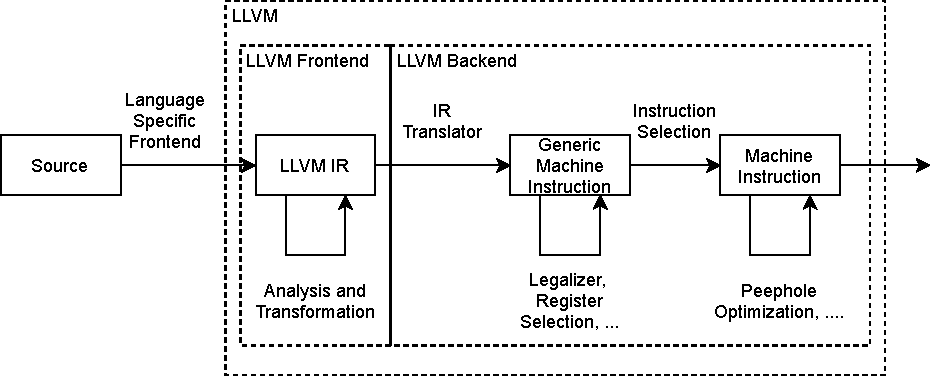
\includegraphics{Images/llvm-intro.pdf}
  \caption{A illustration of LLVM compilation pipeline}
  \label{fig:llvm-intro}
\end{figure}

\begin{figure}
  \centering
  \lstinputlisting[
    language=LLVM,
    basicstyle=\linespread{0.8}\small\ttfamily,
    numbers=left
  ]{Code/adler32.ll}
  \caption{Adler 32 in LLVM}
  \label{fig:adler-32-llvm}
\end{figure}

\paragraph{Register-based IR against stack-based IR}
In WebAssembly, all instructions operate over an implicitly declared stack. For
example, in figure~\ref{fig:adler-32-webassembly} at line $20$, a 32-bit integer
constant instruction, \texttt{i32.const}, will push the constant value on the
stack, and a 32-bit add instruction, \texttt{i32.add} will pop two values off
the stack as left-hand-side and right-hand-side operands accordingly, then push
the sum onto the stack. On the other hand, LLVM utilizes a register-based IR,
which is more similar to what one would expect on a native machine. In
figure~\ref{fig:adler-32-llvm}, each value for example, \texttt{\%0},
\texttt{\%1}, etc is a virtual register. Later in the backend, the register
allocation pass will map the virtual registers into physical registers using
register allocation algorithms.

\paragraph{Control flow, basic block, and $\phi$ instruction}
As we saw in previous sections, WebAssembly has specialized instructions to
manage the program's control flow. On the other hand, LLVM took a more
traditional approach to the problem. In 1991, researchers from IBM introduced
\emph{static single assignment} (SSA) form to ease the difficulty of writing
program analysis and transform passes \cite{ibm-ssa}. In SSA, each value has its
definition exactly once, and hence, the use-definition chain (UD chain) is
trivial to compute. The UD chain presents the relationship between variable
declarations and variable-uses in a graph. It helps the analysis pass to
efficiently pinpoint the information about variables and identify if the
variable declaration is necessary or not. However, in most of the programs,
these information needs to be merged from different control-flows; for example,
in a for-loop, the loop counter may be defined in the loop initialization and on
each loop iteration. The SSA introduces a special kind of instructions, $\phi$
instructions, which explicitly mark the merge of definitions from different
execution paths. LLVM adopts this design principle in its intermediate
representation. In figure~\ref{fig:adler-32-llvm} we have multiple $\phi$
instructions. For example, at line $11$ and $12$, value $\%7$ and $\%8$
represent $a$ and $b$ accordingly. We know that $a$ and $b$ initialized to
$0$ and $1$ upon entry and updated on each iteration from our C implementation.
In the generated LLVM IR, these merges induce $\phi$ instructions. For $a$
($\%7$), if the control flow is from the beginning of the function, we set its
value to $1$, and on the other hand, if the control flow is from the loop
iteration, we update its value accordingly. The different paths inducing a
$\phi$ instruction are indicated by basic block numbers. A basic block groups
the maximum number of instructions without control flow transfer. At line $11$,
we see the $\phi$ instruction merges the definition coming from the $\%2$
which is the entry block and $\%4$. Additionally, $\phi$ instructions must
appear before any other instructions within the same basic block, as they model
the merging of values and do not have any execution semantics.

\paragraph{Memory and load-store instruction}
The last significant difference between WebAssembly and LLVM IR is on the memory
and its related instructions. As we discussed earlier, a WebAssembly module can
have access to multiple linear memories \footnote{In the current version of
  WebAssembly, only one linear memory is allowed per module}. One might confuse
WebAssembly's linear memory with the concept of address space in LLVM IR. LLVM
IR associates each address with an integer value, namely, the address space.
However, unlike linear memory in WebAssembly, which has no difference between
one and another, the LLVM backend interprets the address space differently for
various architectures. For example, in the PTX backend, a backend target for
Nvidia GPUs, the implicit address space $0$ refers to traditional main RAM, and
address space $4$ represents the address shared by both main RAM and GPU RAM
\footnote{An introduction for PTX backend:
  \\\url{https://llvm.org/devmtg/2011-11/Holewinski_PTXBackend.pdf}}. For most
of the architecture, the implicit address space is the only address space
available to the programmer. Another difference between WebAssembly and LLVM IR
is on the design of load-store instructions. Load store instructions in both
languages have an attribute of alignment. However, LLVM IR interprets this
attribute differently from WebAssembly. In WebAssembly, the alignment attribute
acts as a hint to the runtime environment. If the alignment hint is unsuitable,
the runtime environment should still proceed under a possible penalty in the
performance. However, in LLVM IR, the alignment attribute is a requirement.
Any memory access that violates the alignment attribute will result in a
undefined behaviour, usually a runtime panic. A load-store instruction in LLVM
IR with alignment set to one will never fail. However, it will be significantly
less efficient as the backend will likely generate byte-wise load and
concatenation instructions.

We visited some of the background information that helps with understanding the
thesis in this chapter. In the next chapter, we will start from the beginning of
the system implementation, the WebAssembly parsing and validation frontend.
\chapter{Frontend}

This chapter describes the frontend of SableWasm. The front end consists of two parts, the bytecode parser and validation pass.  WebAssembly is a continuously evolving language, and its community might add new instructions in the future. Hence, the parser and the bytecode validation phase's design closely follow WebAssembly's specification and modular to ensure the framework's extensibility. A read-only view of the module structure provides additional functionality. The parser and validation phase design focuses on performance, both in execution time and memory footprint. 

\section{Bytecode Parser}
One of WebAssembly's binary format design goals is simple to parse. Although there are existing open-source bytecode parsing and validation library available when writing the thesis, such as WABT \footnote{WebAssembly Binary Toolkit: \url{https://github.com/WebAssembly/wabt.git}} provided by the WebAssembly community, there is no suitable library at the time when the project starts. Thus, for SableWasm, we implement our bytecode parsing frontend instead. The bytecode parser consists of three components, byte-source reader, WebAssembly bytecode parser and parser delegate. This section will give a brief description of each component, and figure~\ref{fig:sablewasm-parser} presents a general illustration of the parser's design.  

\begin{figure}
  \centering
  \includegraphics[width=\textwidth]{Images/sablewasm-parser.pdf}
  \caption{A illustration of SableWasm parser}
  \label{fig:sablewasm-parser}
\end{figure}

\paragraph{Byte-source Reader}
The byte-source reader consists of two parts, a byte-buffer reader and a WebAssmebly reader. The byte-buffer reader provides essential functionalities such as read and skips. Additionally, the byte-buffer reader also needs to support rewind and barrier. Any out of bound access, either beyond the barrier or byte stream exhausted, the byte-buffer reader will signal via exceptions. On the other hand, the WebAssembly reader provides a richer interface to the parser, such as decode LEB-128 encoded integers and parsing WebAssembly value types. The WebAssembly reader is also responsible for validating the result before passing it to the parser. In the case the result is invalid, the reader throws exceptions similar to the byte-buffer reader.

\paragraph{WebAssembly Parser}
WebAssembly parser is the kernel part of the parsing framework. As we discussed earlier in the chapter, one of the primary design goals of the framework is its extensibility. Hence, the SableWasm parser is modular and consists of three parts, parser core, custom section parser and instruction extension parser. The grammar for WebAssembly binary representation is quite simple, and hence, the parser core implements a simple top-down recursive descent parser with a single byte look-ahead.

\emph{Custom sections} are a special section defined in the WebAssembly standard. They are essentially a binary data chunk tagged with a string name. How to interpret the binary data is different from one to another. These custom sections can either be standardized by the community or defined specific to a toolchain. In this project, we implement two custom sections standardized by the WebAssembly working group, namely \emph{Name} section and \emph{Producer} section. The \emph{Name} section gives human-readable names to functions and their local variables that help program debugging. The specification does not require these names to be the same as the import or export names. There is no direct support for more detailed debug information encoding in WebAssembly, at the time of thesis writing. However, extensions are working on this problem, such as DWARF for WebAssembly \footnote{DWARF for WebAssembly: \url{https://yurydelendik.github.io/webassembly-dwarf/}}; on the other hand, the \emph{Producer} section is relatively simple. It only encodes the information about the toolchain that generates the module, such as the toolchain name and version. All custom section parsers in SableWasm derived from the base class \texttt{CustomSection}. The parser core will dispatch the binary chunk to search custom section parser based on the name tag. Each custom section parser manages its results and does not communicate to the parser delegate directly. Instruction extension parsers focus on another different aspect of the WebAssembly module.

In the background section, we have visited several extensions that merged to the WebAssembly specification. A quick reminder, WebAssembly extensions can insert or modify the instructions defined in the minimum-viable-product (MVP)  specification. The SableWasm WebAssembly parser employs instruction extension parsers to address this problem. When the parser intends to parse an instruction, it will iterate over all its instruction extension parsers in a chained manner. If the instruction opcode is not recognized by any registered instruction extension parser nor in the minimum-viable-product specification, the parser will signal the error by throwing an exception. 


\section{WebAssembly Bytecode Representation}

\section{WebAssembly Bytecode Validation}

\section{Performance Evaluation}
\chapter{Middle-level Intermediate Representation}
\label{chapter:mir-design}

This chapter describes SableWasm's middle-level intermediate representation
(MIR), which has a critical role in the entire compilation pipeline. The MIR
acts as a middle ground between the WebAssembly bytecode frontend and various
possible backends. Currently, SableWasm only implements one backend that
utilizes the LLVM compilation framework, but adding more backend support should
not require significant modification on the MIR. It also implements an
analysis and transformation framework where we perform several optimizations
over the MIR. We will first go over the overall design of the MIR, and
later move to the translation rules and analysis framework in the
chapter~\ref{chapter:mir-translation-optimization}. \\[12pt]


In the previous chapters, we covered the design of WebAssembly bytecode. A quick
reminder, WebAssembly is a stack-based intermediate representation (IR) where
all instructions operate over an implicitly declared operand stack. There are
several advantages of a stack-based IR. Perhaps the most important one is its
portability. A stack-based IR makes fewer assumptions on the machine than a
register-based one. One can even provide an implementation for a hypothetical
device with only one register. Another advantage is the code size. Experiments
show that, in general, a stack-based IR is smaller in size than its
corresponding registered version \cite{stack-and-register-vm}. When designing a
binary format that ships executables over the internet, the stack-based IR seems
to be a better choice for WebAssembly.

Nevertheless, there are no silver bullets: a stack-based IR design also has its
drawbacks. One of them is the difficulty faced when performing code analysis and
transformation over the module. As for each instruction, its operands implicitly
come from the stack; the value use-definition relationship between instructions
is not apparent to the analysis, and recovering such connection between
instructions from the IR is not a trivial task.

\begin{figure}
    \centering
    \lstinputlisting[
        language=SableWasmMIR,
        basicstyle=\linespread{0.8}\ttfamily,
        numbers=left
    ]{Code/4.MIR/fibonacci.mir}
    \caption{Fibonacci in translated SableWasm MIR}
    \label{fig:mir-fibonacci}
\end{figure}

On the other hand, we have the register-based intermediate representation,
commonly abstracted to assume an infinite number of registers and requiring a
register allocation algorithm to map them to actual, physical registers. For
each instruction in register-based IR, it has its operand encoded in the
instruction. Hence, the use-definition relationship will become explicit to the
analysis and transformation.

The main design goal for SableWasm MIR is to provide an analysis platform for
the entire compiler system. Thus, we implement our MIR as an infinite register
machine. We also take a traditional approach in various other aspects. For
example, instead of using the structured control flow similar to what
WebAssembly offers, we use \emph{control-flow graphs} (CFGs) to represent the
relationship between basic blocks. The SableWasm MIR is also in
\emph{single static assignment} (SSA) form \cite{ibm-ssa}, as covered in the
background chapter. The design for instruction and module-level entities in
SableWasm MIR is quite similar to what WebAssembly instruction offers. One can
view the SableWasm MIR as a mixture of the target LLVM intermediate
representation and the source WebAssembly bytecode. We also adopt several design
features from LLVM IR into MIR, such as automatically managed use-site lists,
which provide each AST node with an efficient way to access their use sites.
In SableWasm MIR, all elements are derived from the base class \texttt{ASTNode}
which implements these features that are helpful later in MIR analysis and
transformation.

Figure~\ref{fig:mir-fibonacci} shows a simple function that calculates Fibonacci
numbers with a recursive method in SableWasm MIR. With the help of the figure,
we will go through the detailed design of SableWasm later in the chapter. We
will first present the module-level entity and their initializer
expressions, such as functions, then move to the design of each instruction
defined in MIR.

\subsection{MIR Module Entities}

\begin{figure}
  \centering
  \includegraphics[width=\textwidth]{Images/4.MIR/module.pdf}
  \caption{SableWasm MIR Module-level entities}
  \label{fig:sablewasm-mir-module}
\end{figure}

SableWasm module-level entities are the top-level elements in a translation module. They are direct implements of the WebAssembly module entities defined in the specification. Figure~\ref{fig:sablewasm-mir-module} presents a general illustration of the SableWasm module-level entities. In this section, we will cover the design of each entity and compare them with its WebAssembly correspondent.

\paragraph{Function}
In figure~\ref{fig:mir-fibonacci}, we have a function definition at line 8. A function declaration in SableWasm provides information about the type, local variables and name. A function definition should satisfy all the requirements of function declaration, and additionally, provides a function body using basic blocks. The design of the function declaration and definition in SableWasm is quite similar to that of WebAssembly. The major difference is how to represent the function body. We will come back to this in the later sections within the chapter. Finally, like other module-level entities, a SableWasm function can optionally have import or export annotations. These annotations provide names for the import and export entries in the WebAssembly module.

\paragraph{Global}
SableWasm's global variable declaration and definition follow the design in WebAssembly. In SableWasm, we relax several of the constrain defined in WebAssembly specification and its extensions. In the SIMD extension proposal, the 128-bit vector type is only suitable within the function body. There is no direct way to pass a vector value to the host environment, as there is a lack of standard representation for 128-bit packed vectors in JavaScript \footnote{This might subject to change in the future. WebAssembly SIMD extension proposal is still in the drafting process.}. In  SableWasm, we treat all primitive types uniformly. Thus, a global variable can contain an integral value, a floating-point value or even a packed SIMD vector. The type for the global variable follows the specification in WebAssembly; it is a pair of value type and constness modifier. In figure~\ref{fig:mir-fibonacci}, we have a global definition at line 6, which contains a mutable 32-bit integral value. All global variable definitions in SableWasm must provide a value initialization via initializer expression, which we covered in the previous section. The rules for import and export annotation on the SableWasm function entities also apply to SableWasm global variables, which we do not show in the example above.

\paragraph{Memory and data}
Memory and Data are implementation for WebAssembly linear memory and its initializer, respectively. One might think that there is no need to separate the memory initializer from the memory entity definition, as in WebAssembly specification, all data section entries must provide a valid linear memory index. In the early version of SableWasm, we indeed adopt such implementation. However, this approach might be subject to a significant change in an extension that might soon merge to the WebAssembly specification. The WebAssembly bulk memory operation extension proposal \footnote{WebAssembly bulk memory operations: \\\url{https://github.com/WebAssembly/bulk-memory-operations}} introduce new instructions, such as \texttt{memory.fill} that direct refers to a data section segment. Moreover, the proposal relaxes the constrain on the linear memory index. Now the index can behave like a flag indicating whether the data segment itself is active or not and no longer serves as a linear memory index. Hence, to make our framework `futureproof', we separate the linear memory declaration from their initializers. Figure~\ref{fig:mir-fibonacci} presents a linear memory definition at line 2. SableWasm memory entities also adopt WebAssembly linear memory type. The type consists of a pair of unsigned integers, indicating the lower bound and upper bound of the memory size in WebAssembly pages. Finally, the memory entity can have import and export annotations similar to other module-level entities in SableWasm. The example above defines a memory with a minimal size of 2 pages, 128KiB, and exports it under `memory'. The example above does not provide any example for data initializers, but they are quite easy to understand. A data initializer is essentially a binary chunk with an initialization offset. They are semantically equivalent to a data section entry in an ELF file.

\paragraph{Table and element} SableWasm table and element entity implements the indirect table and its initializer, namely element segment, accordingly. They follow the simple principle as the memory and data entity in the previous section. Currently, like data segment entry, WebAssembly's element section entry must refer to a valid indirect table via an index. In the future, this may also subject to change. WebAssembly reference types extension proposal \footnote{WebAssembly reference types: \url{https://github.com/WebAssembly/reference-types}} introduce instructions such as \texttt{table.fill} that are able to have direct access to element segment initializers. \texttt{table.fill} instruction is similar to \texttt{memory.fill} defined in the bulk memory operation extension. It will copy a sequence of compile-time defined function pointers into an indirect table at runtime. Thus, when we design our table entity, we also split the declarations from their initializers. The type for table entity is the same as the table type in WebAssembly. It consists of a pair of unsigned integers, indicating the lower bound and upper bound for the number of function pointers stored in the indirect table. In SabelWasm MIR, we treat memory entities and table entities as black boxes, and its concrete implementation is deferred to the backend. The example shown in figure~\ref{fig:mir-fibonacci}, the module defines a table entity at line 4 that stores exactly one function pointers. Note that the table entity does not require users to initialize the value for all entries. The table entity default initializes all entries to null pointers. Finally, the rule for import and export annotation also apply for table entity. However, the element entity is local to the module and can neither export nor import from other modules.

In this section, we cover the design for module-level entities in SableWasm. They are pretty similar to the sections defined in WebAssembly specification. In the next section, we will move the design of SableWasm instructions.
\subsection{MIR Initializer Expressions}

\begin{figure}
  \centering
  \includegraphics[width=0.85\textwidth]{Images/4.MIR/initalizer-expression.pdf}
  \caption{SableWasm MIR Initializer Expression}
  \label{fig:sablewasm-mir-initializer-expression}
\end{figure}

WebAssembly defines a particular form of expression for initialization, namely
constant expressions. They can appear in three locations in the current
specification. First, global variables declaration can contain constant
expression as their initialization values. Additionally, data section entries
and element section entries can have constant expressions as the offsets for
their initialization payload. In SableWasm MIR, we define initializer
expressions that act similar to what constant expressions do in WebAssembly.
Figure~\ref{fig:sablewasm-mir-initializer-expression} gives a general
illustration about SableWasm MIR initializer expressions. The initializer
expressions are quite simple. In the current WebAssembly and SableWasm, an
initializer expression can be either a constant value or refer to an imported
global via \texttt{GlobalGet} instruction. Hence, in principle, currently,
a SableWasm MIR initializer expression is essentially a single instruction. In
the future, one may generalize such constraints by allowing more complex
constructs in initializer expressions.

\paragraph{Constant}
The \texttt{Constant} instruction represents a single constant value for the
initializer expression. In WebAssembly, a constant value can be one of the
following: a 32-bit or 64-bit integer, a floating-pointer number, or a 128-bit
SIMD vector \footnote{With WebAssembly SIMD128 extension}, and the specification
encodes the type within the instruction opcode. Hence, there are multiple
instructions in WebAssembly to introduce a constant. In SableWasm, we do not
encode the type into the opcode, and \texttt{Constant} instruction is the only
instruction that takes care of the task. In figure~\ref{fig:mir-fibonacci}, we
have a constant initializer at line 6 that initializes the value of the global
to a 32-bit integer with a value that equals 66560. When querying the type of a
\texttt{Constant} instruction, SableWasm will infer it according to its payload
constant.

\paragraph{GlobalGet}
The \texttt{GlobalGet} instruction is exactly same as the WebAssembly's
\texttt{global.get} in terms of execution semantics. The WebAssembly
specification allows any initializer expression to refer to an imported
\footnote{This might subject to change in the future version of WebAssembly}
global value. As these values are initialized before entering the module,
reading their value is always valid during module initialization. The example
in figure~\ref{fig:mir-fibonacci} does not provide an example of
\texttt{GlobalGet} as an initializer expression, as they are less frequently
used compared to constant initializer expression, especially for global values.
However, in some ABI implementations, data section entries and element section
entries require reading from global values serving as base pointers. SableWasm
also infer the type for \texttt{GlobalGet} initializer expression in a similar
fashion as \texttt{Constant}. In this case, the type of instruction is the same
as the referred global variable without the `constant' modifier.

In this section, we covered the design and implementation of initializer
expressions in SableWasm. They are pretty simple in the current design. We will
now move to the next part in the SableWasm design, the MIR instructions.
\subsection{MIR Instructions}

SableWasm MIR uses control-flow-graph (CFG) based representations in static-single-assignment (SSA) form to represent code body in function definitions. We have provided an introduction to CFG and SSA in the background chapter. Here is a quick recap. CFG splits the control flow within the function into basic blocks. A basic block represents the most extended instruction sequence without control flow transfer, such as branching. Note that for function calls, we take a similar approach that LLVM adopted. We will come back to this in detail later in the section. Additionally, SSA requires that all values must have a unique definition site. Hence, in SSA form, the use-def chain is trivial to compute, while in a traditional CFG, one would need to extract from the graph with the help of reaching definition analysis. SableWasm instruction set is similar to WebAssembly bytecode in terms of semantics for most of the instructions. However, it operates over an infinite register machine instead of a stack-based machine. We also want to keep the size of the SableWasm instruction minimal. Hence, some of the instruction has different semantics compared to the counterpart appears in the WebAssembly specification. In this section, we will cover the design and implementation of SableWasm instructions. The following section will cover the translation strategy between WebAssembly bytecode and the SableWasm instruction set and instruction reduction rules.  Figure~\ref{fig:sablewasm-mir-inst} provides a general illustration of the design of the SableWasm instruction set. The SableWasm instruction sets can currently cover all the instructions set defined in WebAssembly specification, along with several extensions such as multivalue and SIMD vector operations.

\begin{figure}
  \centering
  \includegraphics[width=0.8\textwidth]{Images/4.MIR/sablewasm-instruction.pdf}
  \caption{SableWasm MIR Instructions}
  \label{fig:sablewasm-mir-inst}
\end{figure}

\paragraph{Terminating instructions}
As we discussed above, SableWasm split the function control flow into basic blocks, which contain the maximum amount of consecutive instructions without control flow transfer. In addition, SableWasm, similar to many other SSA form instruction sets, defines a particular group of instructions called terminating instructions. These instructions signal a control flow transfer out of the current basic block, and they must only appear as the last instruction in any given basic block. SableWasm defines four different terminating instructions: unreachable, unconditional branching, conditional branching and table branching. If the control flow reaches a \texttt{unreachable} instruction, the runtime system will signal a runtime panic. The \texttt{unreachable} instruction in SableWasm is identical to its counterpart in WebAssembly in terms of semantics. The \texttt{Unconditonal} instruction is an unconditional control flow transfer, as the name suggests. It refers to a basic block as the operand. At runtime, the instruction will always transfer the control flow to the target basic block. \texttt{Unconditional} is similar to the \texttt{br} instruction defined in WebAssembly specification. On the other hand, \texttt{Conditional} is a conditional branching. It takes a value and two basic blocks as its operands. At runtime, the instruction will compare the value against integral value zero. If the value equals zero, the instruction will transfer the control flow to the `false' basic block, otherwise, to the `true' basic block. SableWasm's \texttt{Conditional} instruction is similar to \texttt{br.cond} defined in WebAssembly. The last terminating defined in SableWasm is \texttt{Switch}. \texttt{Switch} instruction is comparable to the \texttt{br.table} instruction in WebAssembly. The instruction takes a value, a list of basic blocks, and a default branching basic block as its operands. At runtime, \texttt{Switch} will interpret the value as an integral value and dispatch accordingly. If the value is within the branching list's range, it will redirect the control flow to the basic block referred to by the index. Otherwise, \texttt{Switch} will transfer the control flow to the default basic block.

\paragraph{Function call}
In SableWasm, we provide two instructions for function calls defined in WebAssembly specification, direct function calls and indirect function calls. \texttt{Call} defines a direct function call where the callee is known at compile time. It takes a function as callee and a list of arguments as operands. On the other hand, \texttt{CallIndirect} defines an indirect function call. It implements the indirect function call protocol defined in WebAssembly specification. A quick reminder, in WebAssembly, an indirect function call takes an indirect table, the table index, the expecting function type and a list of values as arguments. At runtime, the system should first check if the index is valid for the indirect table and fetch the function pointer and its actual signature accordingly. Then, the system should compare the signature against the expecting type. If the signature matches the type, the runtime system will transfer the control flow to the function referred to by the function pointer. Implementing the signature verification mechanism is backend-specific; we will return to this topic in the next chapter. Note that we do not treat function call instructions as terminating instructions, even transferring the control flow to other locations. In SableWasm MIR, we follow the design that appeared in LLVM intermediate representation. It is guaranteed that the control flow will continue to the next instruction for function call instructions. Hence, from the basic block's local point of view, their control flow is pre-determined, and there is no difference compared to other non-terminating instructions.

\paragraph{Local and global variable access}
In WebAssembly, instructions have access to locals defined by its parent function and global variables defined by its enclosing module. SableWasm defines getter and setter instruction for both local and global variables to implement the specification. Their semantics are the same compare to WebAssembly's counterparts. We will skip the detail here, but one can consult the WebAssembly specification for detailed information.

\paragraph{Numerical operations}
In SableWasm, we classify the numerical operations into three different categories, the \texttt{Compare} instructions, \texttt{Unary} instructions, and \texttt{Binary} instructions. The \texttt{Compare} instructions implements the comparison between values, such as `equal to'. They always yield a 32-bit integer as WebAssembly specification suggests. The \texttt{Unary} and \texttt{Binary} implements , as their name suggests, unary and binary operations between values. The result of \texttt{Unary} and \texttt{Binary} instruction is dependent on the opcode. On the other hand, we can also orthogonally classify the instructions into integer, floating-point and packed integer and packed floating numbers. Note that in MVP WebAssembly, there are only integer and floating-point value operations; the SIMD operation extension proposal adds the packed value operation to the instruction set. In the WebAssembly SIMD extension proposal, the vector value does not store its shape information in the types. Instead, the packed value instructions' opcodes keep track of the shape of the vector values, which leads to the blot of instruction opcodes. In SableWasm, we separate the instruction opcode from the vector shape. For each of the packed value operations, it must have either a \texttt{SIMD128IntLaneInfo} or \texttt{SIMD128FPLaneInfo}. Figure~\ref{fig:sablewasm-mir-inst} shows all the class of numerical operations defined in SableWasm. For detailed opcode of each numerical instruction class, we include them in the thesis appendix.

\paragraph{Load and store}
\texttt{Load} and \texttt{Store} instruction provides access to the linear memory for SableWasm MIR. Although in the current version of WebAssembly, the module can contain at most one linear memory. All load and store implicitly refer to this linear memory \footnote{This subject to change in the future version of WebAssembly.}. \texttt{Load} instruction takes a linear memory and an integer value as operands. At runtime, the value will treat as the address (or offset) respective to the start of the linear memory, and the instruction yields to fetched result. In WebAssembly, the \texttt{load} instruction associates with a type and an extension method. For example, \texttt{i32.load8\_s} load an 8-bit integer from the linear memory, and then signed extends the fetched byte into a 32-bit integer. In SableWasm, \texttt{Load} instruction only associates to an integer value, namely the load width. The load width must equal to or smaller than the load type's width. Also, SableWasm \texttt{Load} always perform zero-extension on loaded value. Hence, when translating WebAssembly's sign-extended load into SableWasm's \texttt{Load}, one must combine the load instruction with a cast instruction. We will come back to this later in the chapter. \texttt{Store} instruction also associate with a store width. Like the load width defined for \texttt{Load} instruction, store width must also be equal to smaller than the store value type's width. At runtime, the system will first perform bit truncate to the value and then store the result into the linear memory. One may notice that in SableWasm, we erase the alignment attribute and offset attribute defined in WebAssembly. Currently, we do not support alignment hints from the WebAssembly module. In SableWasm, the load and store always have the alignment requirement of one byte. This implies that the load and store can happen anywhere in the linear memory, which corresponds to WebAssembly's linear memory specification.

\paragraph{Linear memory manipulation}
WebAsseembly specification defines three instruction can manipulate linear memories, such as \texttt{memory.size}, \texttt{memory.grow}. Like the \texttt{load} instruction we covered in the previous paragraph, all these instructions operate over the implicitly defined unique linear memory within the module. In SableWasm, we provide similar \texttt{MemoryGrow} and \texttt{MemorySize} instruction. The semantics of the SableWasm's memory manipulation instruction is the same as their WebAssembly counterparts, except that the linear memory needs to be explicitly stated. In SableWasm, we introduce a special instruction, \texttt{MemoryGuard} which is an explicit memory boundary check. In WebAssembly, all \texttt{load} and \texttt{store} instruction need to check for linear memory out of bound error before access. SableWasm separates the bound check from the memory access. One advantage of this is that one may implement static memory bounds check elimination optimization over SableWasm MIR. Additionally, one backend may provide different strategies for handling boundary checks, such as utilizing invalid virtual memory pages with the operating system's help. In this case, we only need to modify the translation pattern for \texttt{MemoryGuard}. \texttt{MemoryGuard} takes a linear memory and an integer value as the operand. It also associates with an integer immediate, known as guard width. At runtime, the system will perform a boundary check over the linear memory starting from the given address to determine if it contains at least a given number of bytes ahead. If there are not enough bytes available, the system should signal a runtime panic.

\paragraph{Pack and Unpack}
WebAssembly multivalue specification \footnote{WebAssembly Multi-value Proposal: \url{https://github.com/WebAssembly/multi-value}} relaxes the constrains on the function type. Functions now can return multiple values instead of at most one value. To support these features, we introduce \texttt{Pack} and \texttt{Unpack} instructions, along with extending WebAssembly's type system. \texttt{Pack} instructions group multiple values into an ordered tuple, while the \texttt{Unpack} reverse the operation by retrieving the value from tuples by index. In the case where a function returns multiple values, we use a tuple instead. SableWasm treats tuples as a first-class values; however, currently, tuples cannot be recursive. We will come back to this later in the chapter when we visit the type systems of SableWasm MIR. The index of the \texttt{Unpack} must be an immediate value in the current version of SableWasm MIR and is verified at compile time.

\paragraph{Vector operations}
In the previous paragraph, we introduce the numeric operations defined in SableWasm MIR. However, several instructions does not fix into neither \texttt{Unary} nor \texttt{Binary} instructions. Hence, to faithfully support the SIMD operations introduced by the extension proposal, we add four vector-specific operations into SableWasm MIR. They are \texttt{VectorSplat}, \texttt{VectorExtract}, \texttt{VectorInsert} and \texttt{VectorByteShuffle}. \texttt{VectorSplat} will broadcast the operand value to all lanes in the result vector. SableWasm MIR defines vector splat operation for both packed integer vector and packed floating-point vector. \texttt{VectorExtract} is similar to the \texttt{extractelement} defined in LLVM intermediate representation. It takes a vector as the operand and also associates itself with an immediate integer value. At runtime, the system extracts the value of the given lane and yields as a result. \texttt{VectorInsert} is similar to \texttt{insertelement} defined in LLVM. It will replace the vector operand with a given value and yields the updated vector as a result. Note that in the WebAssembly SIMD extension proposal, there are more instructions defined that modify the individual lane value of the vector, such as \texttt{V128Load32Lane} which loads a 32-bit value into a specific lane within the vector. In this project, we would like to keep our instruction set simple; hence, these instructions are reduced into multiple SableWasm MIR instructions. We will come back to this later in the chapter when we discuss the instruction reduction rules. The last instruction we introduced is the \texttt{VectorByteShuffle}. \texttt{VectorByteShuffle} is similar to \texttt{shufflevector} defined in LLVM, except that it operates on bytes instead of lanes. Currently, the \texttt{VectorByteShuffle} only operates over an array of immediate integer values. Compare to the lane shuffle semantics, byte shuffle semantics provides more precise control over the result value. One can trivially simulate the lane shuffle with byte shuffle. The WebAssembly SIMD extension proposal only defines shuffle for \texttt{i8x16}, which corresponding to the byte shuffle semantics. However, in the future, if another shape vector supports shuffle operation, one can generalize the implementation with minimal modification.

\paragraph{Cast}
\texttt{Cast} models the conversion of values to their equivalent form in other types. One may argue that \texttt{Cast} instruction is just a numerical \texttt{Unary} operations, and it is partially true. However, in SableWasm MIR, we would like to group the conversion and extension instructions into their groups; and later in the analysis phase, we can focus on numerical operations in the case of \texttt{Unary}.  In SableWasm MIR, we do not distinguish between value conversion and value extension. We treat signed and zero extensions as a kind of value conversion. The \texttt{Cast} instruction takes a single value as the operand, and it associates itself with a cast opcode. At runtime, it will perform the conversion according to the opcode, and if the result cannot be accurately represented in the target type, the system should signal an error. The cast opcodes are direct implementations of their WebAssembly counterparts, and we will skip the detail here. One may refer WebAssembly specification for more details.

\paragraph{Intrinsic}
The last SableWasm MIR instruction we are going to cover in this chapter is the \texttt{Intrinsic} instructions. Most WebAssembly instructions can be represented by using the SableWasm MIR instructions, which we covered earlier in the section. However, there are still several corner cases. For example, the WebAssembly SIMD extension proposal defines Q-format rounding multiplication, a type of fix-point multiplication, for packed 16-bit integers. Another example is the \texttt{swizzle} operation. A \texttt{swizzle} operation is similar to a shuffle operation, except that it takes another vector as the shuffle indices vector instead of an array of immediate integer values. These operations are only defined for a specific vector shape and will introduce unneeded complexity to the SableWasm MIR if we generalize them to all possible vector shapes. Hence, here we group these instructions as the \texttt{Intrinsic} instructions. There is no direct mapping to LLVM instruction, even with the intrinsic functions provided by the framework for most of them. Hence, the backend is encouraged to support these instructions with runtime library routines.

In this section, we discussed the design of the SableWasm MIR instruction set, and in the next section, we will move the translation strategy between WebAssembly and SableWasm MIR.


\chapter{Middle-level Intermediate Representation Translation and Optimization}
\label{chapter:mir-translation-optimization}

The previous chapter presented the SableWasm middle-level intermediate
representation (MIR), a static-single-assignment (SSA) control flow graph (CFG)
representation of a WebAssembly program. This chapter focuses on the translation
strategy used when lowering WebAssembly into the SableWasm MIR. We will first
start by presenting the translation patterns used and then discuss the analysis
and optimization framework.

\section{Translating WebAssembly to MIR}
\label{section:mir-translation}

In this section, we will cover the translation between WebAssembly bytecode and
SableWasm MIR. We have covered the design of SableWasm MIR instructions
previously. One may notice that for most of the instructions, especially for the
numerical operations, SableWasm MIR shares the same semantics as WebAssembly.
Hence, the translation rules for these instructions are pretty trivial, and we
will not cover them in detail in this section. Instead, this section will focus
on the translation rules for the structured control flow constructs and
WebAssembly instructions that require reduction during translation.

\subsection{Structured-Control-Flow Construct}

Translating from stack-based IR to register-based IR is not trivial, especially
when non-linear control flow structures appeared. This problem appeared in many
runtime system implementations, such as Numba \cite{numba}, a just-in-time (JIT)
compiler for Python. Usually, one needs some algorithm to recover the control
flow structure from annoying jump instructions. Luckily, in WebAssembly, we can
translate the stack-based bytecode into register-based basic blocks in linear
time, thanks to the structured-control-flow constructs and their validation
rules defined in WebAssembly. In this section, we will cover the translation
pattern used for WebAssembly's structured-control-flow constructs, namely
\texttt{block}, \texttt{if} and \texttt{loop}.

\begin{figure}
  \centering
  \includegraphics[width=\textwidth]{Images/4.MIR/translate-block.pdf}
  \caption{WebAssembly \texttt{block} translation pattern}
  \label{fig:translate-block}
\end{figure}

\begin{figure}
  \centering
  \includegraphics[width=\textwidth]{Images/4.MIR/translate-if.pdf}
  \caption{WebAssembly \texttt{if} translation pattern}
  \label{fig:translate-if}
\end{figure}

\paragraph{Block}
In the background chapter, we provide a general illustration of the three
structured-control-flow constructs. As a quick recap, \texttt{block} is the
simplest form of a structured-control-flow construct. It implicitly introduces
a label at the end of its enclosing instructions. A branching instruction
referring to this label will redirect the control flow to the end of the block.
Figure~\ref{fig:translate-block} illustrates the translation pattern for
WebAssembly \texttt{block} in SableWasm MIR. We will first clarify some of the
terminologies we used in the figure, and we will use the same terms later in
the \texttt{loop} and \texttt{if} pattern discussion. \emph{Expr Insert Point}
refer to the starting position for the generated instructions when we
recursively translate the instructions within the enclosing expression of the
\texttt{block} instruction. Furthermore, \emph{Label Insert Point} refer to the
position for generated instruction when we finish the recursive translation and
resume to the parent expression of the \texttt{block} instruction. A \emph{label
  stack entry} is a tuple consisting of a pointer to the landing BB, a list of
$\phi$ nodes expecting merge values, and a pointer to the \emph{label insert
  point}. The translation pattern for \texttt{block} is pretty simple; we
continue on the current BB and prepare the landing BB for the block instruction
as a branch instructions within the expression may refer to the label.
Additionally, to fully support multi-value extension in WebAssembly, we also
need to prepare the $\phi$ nodes in the landing BB. SableWasm generates the
$\phi$ nodes based on the type of the \texttt{block} instruction. WebAssembly
validation ensures that the expression within the \texttt{block} can access
exactly $m$ values from the stack and put $n$ values onto the stack. Finally,
we will append an unconditional branch to the landing BB because in WebAssembly,
if the control flow reaches the bottom of the \texttt{block} expressions, it
will implicitly fall through. For the operand stack, we will first pop $m$
values from the stack as \texttt{block} instruction's type suggests and push the
$\phi$ nodes as the result values. Now we need to set up the operand stack for
our the expression contained within the block. Again, due to the WebAssembly
validation rule, we need to insert a boundary before continuing.
Figure~\ref{fig:translate-block} represents this with the bold line in the
result operand value stack.


\paragraph{If}
The next control-flow structure defined WebAssembly is \texttt{if}.
WebAssembly's \texttt{if} is an expression instead of a statement that appears
in many other languages such as C. The \texttt{if} expression can yield some
values indicated by its type. Figure~\ref{fig:translate-if} illustrates the
translation patterns in SableWasm. There are two types of \texttt{if}
instruction defined in WebAssembly specification. The first case is a `partial'
\texttt{if} instruction, where it only contains the `true' branch. From
WebAssembly validation rules, it's easy to show that the only possible type is
\texttt{[i32]->[]}, even with the multi-value extension proposal. This implies
that the expression within the \texttt{if} instruction must start with an empty
operand stack. Hence, the translation pattern for the partial \texttt{if} is
quite straightforward: we only need to pop the condition value from the operand
stack and construct a conditional branch based on this value in the current BB.
On the other hand, we also have `full' \texttt{if} instructions with both `true'
expression and `false' expression. The validation rules ensure that both
expressions must have the same type. The translation pattern is more complex
compare to that of a `partial' \texttt{if}. In this case, we have to prepare the
landing BB similarly to what we did for the \texttt{block} construct. We need to
generate $n$ $\phi$ nodes for data-flow mergers from the true branch, the false
branch, and any possible branching instruction within both nested expressions.
Similarly, we need to pop $m$ values from the stack for operand values stack and
then push $n$ $\phi$ nodes. And, within both nested expressions, push $m$ values
back to the stack.

\begin{figure}
  \centering
  \includegraphics[width=\textwidth]{Images/4.MIR/translate-loop.pdf}
  \caption{WebAssembly \texttt{loop} translation pattern}
  \label{fig:translate-loop}
\end{figure}

\paragraph{Loop}
The last control-flow structure defined in WebAssembly is \texttt{loop}.
Figure~\ref{fig:translate-loop} gives a general illustration of SableWasm's
translation pattern for \texttt{loop} instructions. Similar to the `partial'
\texttt{if} we discussed in the previous paragraph, one can show that, under
WebAssembly's validation rules, the parameter types for the \texttt{loop}
instruction must equal to the result types. The \texttt{loop} instruction is
similar to the \texttt{block} instruction, except that if any branching
instruction refers to it, the branching instruction should transfer the control
flow to the start of the expression within the instruction instead of the end.
Thus, we need to prepare a standalone basic block for the nested expression in
\texttt{loop}, along with the $\phi$ nodes to merge value on each loop
iteration. Note that we also introduce $\phi$ nodes in the landing BB. One may
argue that there is no need for these $\phi$ nodes, as only one block can reach
the loop exit and no value merging will occur. Indeed, these $\phi$ nodes will
always be trivial $\phi$ nodes, which have only one possible value inflow.
However, this is due to the limitation of our translation framework.

In this section, we discussed the translation patterns for WebAssembly
structured control-flow constructs. Thanks to WebAssembly validation rules, the
types for these structured control-flow instructions explicitly mark value
merging and imply possible $\phi$ nodes. Furthermore, one can show that the
control graph generated above is indeed in SSA form. However, the directly
generated control flow graph is not easily understandable by users. This mainly
comes from two facts. First, the WebAssembly-targeting compiler may generate
awkward patterns to fit in the structured control-flow constructs. Second,
SableWasm translation patterns for structured-control flow constructs are not
optimal.
\subsection{Instruction Reduction}

This section will cover the instruction reduction rules used when lowering
WebAssembly bytecode to SableWasm MIR. In the background chapter, we mentioned
that one of WebAssembly's design goals is to be as compact as possible. Thus,
when the community designed the WebAssembly instruction set, they fused several
typical instruction sequences into single instructions. For example, SIMD vector
operation extension defines \texttt{v128.load8x8\_s} which first load 8
8-bit integers into a vector, and then sign-extends them into 16-bit
integers. Another example will be \texttt{v128.load32\_lane} which loads a
32-bit value, either a 32-bit integer or a single-precision floating-point
number into a given vector. Such design is understandable for WebAssembly as
binary size does matter when shipping applications over the internet. But, for
SableWasm, a static compiler, we focus more on the size of the instruction set
instead of the size of the intermediate representation. It is harder to write
analysis for a bloated instruction set, as one needs to consider more
instruction cases. Hence, when lowering WebAssembly bytecode to SableWasm MIR,
we replace some WebAssembly instructions with SableWasm MIR instructions
sequences.

\paragraph{Eqz} \quad
\begin{lstlisting}[
    basicstyle=\linespread{0.7}\small\ttfamily, 
    language=SableWasmMIR, 
    mathescape=true]
[..., %n i32] i32.eqz $\Longrightarrow$ %t0 = i32.const 0; %t1 = int.eq %n %t0
[..., %n i64] i64.eqz $\Longrightarrow$ %t0 = i64.const 0; %t1 = int.eq %n %t0
\end{lstlisting}
WebAssembly defines a unary \texttt{eqz} operations for all integer values. As
the name suggests, \texttt{eqz} compares the operand value against zero and
yields one if true, zero otherwise. In SableWasm MIR, we group all comparison
instructions into the \texttt{Compare} class, and \texttt{eqz} does not fit into
the class as it is not a binary operation. Hence we rewrite the \texttt{eqz} as
\texttt{Compare} instruction with opcode as \texttt{Eq}.

\paragraph{Load} \quad
\begin{lstlisting}[
    basicstyle=\linespread{0.7}\small\ttfamily, 
    language=SableWasmMIR, 
    mathescape=true]
[..., %base i32] i32.load offset=%offset align=%align $\Longrightarrow$
    %addr = int.add %base %offset
    memory.guard %mem %addr 4
    %t0 = load.32 i32 %mem %addr
[..., %base i32] i32.load16_s offset=%offset align=%align $\Longrightarrow$
    %addr = int.add %base %offset
    memory.guard %mem %addr 2
    %t0 = load.16 i32 %mem %addr
    %t1 = cast i32.extend.16.s %t0
[..., %base i32] i32.load16_u offset=%offset align=%align $\Longrightarrow$
    %addr = int.add %base %offset
    memory.guard %mem %addr 2
    %t0 = load.16 i32 %mem %addr
\end{lstlisting}
In the SableWasm instruction design section, we introduced the \texttt{Load} and
\texttt{MemoryGuard} in SableWasm MIR. A quick recap, SableWasm MIR
\texttt{Load} instruction, compare to its WebAssembly counterpart, assumes
access is in-bound, does not support offset attribute, and always performs
zero-extension on partial loads. Hence, to properly support WebAssembly's
\texttt{load} instructions, we need to reduce them with the strategy shown
above. For load instructions that do not require value extensions, such as
\texttt{i32.load}, we first calculate the actual starting address, perform a
memory boundary check with \texttt{MemoryGuard}, and then perform the memory
read. On the other hand, for a partial load operation, we need first to perform
the load operation using the same protocol as a normal load. Then, if a sign
extension is needed, we will add its corresponding cast instruction. In the
example above, we demonstrate this with WebAssembly's \texttt{i32.load16\_s}.
In this case, SableWasm appends a \texttt{Cast} instruction with opcode
\texttt{i32.extend.16} after the load operation.

\paragraph{Store} \quad
\begin{lstlisting}[
    basicstyle=\linespread{0.7}\small\ttfamily, 
    language=SableWasmMIR, 
    mathescape=true]
[..., %base i32, %val i64] i64.store offset=%offset align=%align $\Longrightarrow$
    %addr = int.add %base %offset
    memory.guard %mem %addr 8
    store.64 %mem %addr %val
[..., %base i32, %val i64] i64.store16 offset=%offset align=%align $\Longrightarrow$
    %addr = int.add %base %offset
    memory.guard %mem %addr 2
    store.16 %mem %addr %val
\end{lstlisting}
Similar to the \texttt{Load} instruction we discussed earlier, the
\texttt{Store} instruction also assumes the memory access is always in range and
does not provide the offset attribute. However, a \texttt{Store} instruction
will always perform truncation instead of extension. Further, the only possible
truncation is the bit-truncation by discarding bits starting from the most
significant bit. The instruction reduction rules for WebAssembly \texttt{store}
instructions is similar to those for \texttt{load} instructions. In the example
above, we demonstrate the rules with \texttt{i64.store} and its partial store
version, \texttt{i64.store16} which only stores the lowest two bytes into linear
memory. SableWasm inserts \texttt{MemoryGuard} instructions in a similar fashion
to \texttt{load} instructions. Note that we do not insert an explicit
\texttt{Cast} instruction to perform the truncation. A \texttt{Store}
instruction will implicitly truncate the value according to the store width; in
this case, it will truncate the 64-bit integer into a 16-bit integer.

\paragraph{SIMD extension proposal reduction rules} \quad
\begin{lstlisting}[
    basicstyle=\linespread{0.7}\small\ttfamily, 
    language=SableWasmMIR, 
    mathescape=true]
[..., %lhs v128, %rhs v128] v128.andnot $\Longrightarrow$
    %t0 = v128.not %rhs 
    %t1 = v128.and %lhs %t0
[..., %lhs v128, %rhs v128] i16x8.extmul_low_i8x16_s $\Longrightarrow$
    %t0 = cast i16x8.extend.low.i8x16.s %lhs
    %t1 = cast i16x8.extend.low.i8x16.s %rhs
    %t2 = v128.int.mul i16x8 %t0 %t1
[..., %lhs v128, %rhs v128] i16x8.extmul_low_i8x16_u $\Longrightarrow$
    %t0 = cast i16x8.extend.low.i8x16.u %lhs
    %t1 = cast i16x8.extend.low.i8x16.u %rhs
    %t2 = v128.int.mul i16x8 %t0 %t1
\end{lstlisting}
The SIMD extension proposal introduces approximately 240 instructions into the
WebAssembly instruction set. However, not all of them are simple single
operation instructions. The SIMD extension proposal also follows WebAssembly's
design goal to ensure the compactness of the generated program. The proposal
suggests reduction rules for several SIMD operation instructions, and in
SableWasm, we take advantage of them to reduce the size of the instruction set.
The first applicable instruction is the \texttt{andnot} operation for vectors.
The \texttt{andnot} is equivalent to performing bitwise `not' on the
right-hand-side operand, and then a bitwise `and' operation between the
left-hand-side operand and the temporary result. SableWasm reduces
\texttt{andnot} into a \texttt{not} instruction followed by a \texttt{and}
instruction, as shown in the example above. The second group of reducible
instructions is the \texttt{ExtMul} instructions. The SIMD extension proposal
defines \texttt{ExtMul} for all packed integer vectors except packed 64-bit
integers. They are equivalent to first widening the vector using the appropriate
extension and then multiplying two operands. In the example above, we
demonstrate with \texttt{i16x8.extmul\_low\_i8x16\_s} which performs an
\texttt{ExtMul} operation for packed 8-bit integers. SableWasm implements this
instruction by first performing a sign extension on the lower half of the vector
and multiplying the temporary result as shown above. SableWasm also applies a
similar procedure to \texttt{i16x8.extmul\_low\_i8x16\_u}, except that it uses
a zero-extension in the \texttt{Cast} instruction instead of sign-extension.

\paragraph{SIMD load with zero-padding} \quad
\begin{lstlisting}[
    basicstyle=\linespread{0.7}\small\ttfamily, 
    language=SableWasmMIR, 
    mathescape=true]
[..., %base i32] v128.load32_zero offset=%offset align=%align $\Longrightarrow$
    %addr = int.add %base %offset
    memory.guard %mem %addr 4
    %t1 = load.32 i32 %mem %addr
    %t2 = const v128 0
    %t3 = v128.int.insert i32x4 0 %t2 %t1
\end{lstlisting}
The WebAssembly SIMD extension proposal also introduces many variations of load
operations. The first variation is the `zero-padding' load operation. The
`zero-padding' load is equivalent to loading a scalar from the linear memory and
then inserting it into a zero-initialized vector. We demonstrate this with the
example above. We first use the protocol we discussed above to load a scalar
32-bit integer. Then, we insert it into a zero vector using
\texttt{VectorInsert} instruction. The WebAssembly SIMD extension proposal
defines `zero-padding' load operations for all packed integers and
packed float-point numbers. The reduction rules for them are similar to the
pattern above.

\paragraph{SIMD load and splat} \quad
\begin{lstlisting}[
    basicstyle=\linespread{0.7}\small\ttfamily, 
    language=SableWasmMIR, 
    mathescape=true]
[..., %base i32] v128.load32_splat offset=%offset align=%align $\Longrightarrow$
    %addr = int.add %base %offset
    memory.guard %mem %addr 4
    %t1 = load.32 i32 %mem %addr
    %t2 = v128.int.splat i32x4 0 %t1
\end{lstlisting}
The second variation of SIMD vector load is the `load-and-splat' load operation.
This type of load operation is a combination of scalar load operation and vector
splat operation. It first loads a scalar from the linear memory and then
broadcasts the value to all vector lanes. SableWasm uses a similar reduce rule
compared to the `zero-padding' load operation, except that instead of inserting
the scalar into a zero-initialized vector, we use \texttt{VectorSplat} to
broadcast it. The example above demonstrate this with
\texttt{v128.load32\_splat}. Similar to the `zero-padding' load operation,
`load-and-splat' is defined for all packed integers and packed float-point
numbers.

\paragraph{SIMD load lane} \quad
\begin{lstlisting}[
    basicstyle=\linespread{0.7}\small\ttfamily, 
    language=SableWasmMIR, 
    mathescape=true]
[..., %base i32, %vec v128]
v128.load32_lane offset=%offset align=%align lane=%lane $\Longrightarrow$
    %addr = int.add %base %offset
    memory.guard %mem %addr 4
    %t1 = load.32 i32 %mem %addr
    %t2 = v128.int.insert i32x4 %lane %base %t1
\end{lstlisting}
The next variation of the SIMD vector load operation is the `load-lane' load
operation. The example above demonstrates the procedure with a sample of
WebAssembly's \texttt{v128.load32\_lane} which reads a 32-bit integer from
linear memory and inserts it into a specific lane of a given vector. SableWasm
first lowers the load semantic using the same protocol as we discussed above and
then inserts to the given vector using the \texttt{VectorInsert} instruction.
Again, the WebAssembly SIMD extension proposal defines `load-lane' load
operation for all shapes of packed integers and floating-point numbers. In
WebAssembly SIMD load operation variations, one may already notice that we only
have a width associated with them instead of types. This is because WebAssembly
SIMD operations do not distinguish the shape of the vector. Hence, there is no
difference in loading a 32-bit integer and a single-precision floating number,
as they both consume 32-bit storage. But in SableWasm, we distinguish between
packed integers and packed floating-point numbers for the SIMD instruction shape
record. On the other hand, SableWasm also erases shape information from the
vector value, and it is the responsibility of the instruction to interpret the
value correctly. Thus, when we perform a load operation, we always assume that
we are loading packed integers. In the examples above, the 32-bit load with
translate to `load a 32-bit integer'.

\paragraph{SIMD load and extend} \quad
\begin{lstlisting}[
    basicstyle=\linespread{0.7}\small\ttfamily, 
    language=SableWasmMIR, 
    mathescape=true]
[..., %base i32] v128.load16x4_s offset=%offset align=%align $\Longrightarrow$
    %addr = int.add %base %offset
    memory.guard %mem %addr 8
    %t1 = load.64 v128 %addr 8
    %t2 = cast i32x4.extend.low.i16x8.s %t1
[..., %base i32] v128.load16x4_u offset=%offset align=%align $\Longrightarrow$
    %addr = int.add %base %offset
    memory.guard %mem %addr 8
    %t1 = load.64 v128 %addr 8
    %t2 = cast i32x4.extend.low.i16x8.u %t1
\end{lstlisting}
The last variation of a load operation is the `load-and-extend' load operation.
It is a combination of partial load and extension on the lower half of
128-bit vectors. In the example above we present examples for
\texttt{v128.load16x4\_s} and \texttt{v128.load16x4\_u}. The previous
instruction loads four 16-bit integers into the lower lanes of the vector and
performs sign-extension on the result to get a packed 32-bit integer vector.
\texttt{v128.load16x4\_u} performs a similar operation, except that it performs
zero-extension instead of sign-extension. A quick reminder, SableWasm MIR
\texttt{Load} instruction can apply to any primitive value type and supports
partial loading by annotating with a smaller load-width. In the case of the
partial load, SableWasm MIR \texttt{Load} always loads bytes starting from the
least significant bit and performs zero-extension on the result. SableWasm takes
advantage of the \texttt{Load} instruction's design when lowering the
`load-and-extend' load operation. In the example above, we partially load a
128-bit vector with a 64-bit value which corresponds to loading four
16-bit integers from the linear memory. Note that this \texttt{Load} instruction
yields a vector of 16-bit integers with four zero values in its higher lanes and
loaded values in its lower lanes. Thus, we only need to perform a \texttt{Cast}
operation with opcode \texttt{i32x4.extend.low.i16x8.s} to reach the desired
result. SableWasm treats \texttt{v128.load16x4\_u} using a similar procedure,
except that it uses zero-extension instead of sign-extension. Finally, like
other load operation variations discussed above, WebAssembly defines the
`load-and-extend' load operation for all packed integer and packed
floating-point numbers.

\paragraph{SIMD store lane} \quad
\begin{lstlisting}[
    basicstyle=\linespread{0.7}\small\ttfamily, 
    language=SableWasmMIR, 
    mathescape=true]
[..., %base i32, %val v128]
v128.store32_lane offset=%offset align=%align lane=%lane $\Longrightarrow$
    %addr = int.add %base %offset
    memory.guard %mem %addr 4
    %t1 = v128.int.extract i32x4 %val %lane
    store.32 %mem %addr %t1
\end{lstlisting}
Similar to the `load-lane' load operation variation, the WebAssembly SIMD
extension proposal also defines direct lane store instruction for 128-bit
vectors. The above example demonstrates the reduced rules for these
instructions. Let's take \texttt{v128.store32\_lane} as example. SableWasm MIR
first calculates the address and sets up a memory boundary check use a protocol
similar to what we have seen above. Then, it extracts the lane value by using
\texttt{VectorExtract} instruction and stores it into linear memory. Like
WebAssembly \texttt{load} instructions, the \texttt{store} instruction does
not distinguish between packed integers from packed floating-point numbers.
In SableWasm, we always assume the store vector is packed integers.


\section{Analysis Framework}
\label{section:mir-opt}

\begin{figure}
    \centering
    \includegraphics[width=\textwidth]{Images/4.MIR/analysis-framework.pdf}
    \caption{SableWasm MIR Analysis and Optimization Framework}
    \label{fig:sablewasm-mir-analysis-framework}
\end{figure}

SableWasm also implements an analysis and optimization framework over its
middle-level intermediate representation (MIR). The framework consists of two
parts, passes and drivers. The SableWasm analysis and transformation framework
only provides essential support for managing passes, compared to other more
advanced frameworks, such as McSAF\cite{mcsaf}, an optimization framework for
MATLAB language. Figure~\ref{fig:sablewasm-mir-analysis-framework} illustrates
the current state of the framework in SableWasm. Currently, we implement three
different drivers. \texttt{SimpleModulePassDriver} accepts module passes and
operates on the module level. At the time of thesis writing, we haven't explored
inter-procedural analysis for SableWasm MIR in detail, and the only module pass
implemented is the pretty-print pass. In the future, one can add additional
inter-procedural analyses to SableWasm, by implementing the \texttt{ModulePass}
interface. The second driver is the \texttt{SimpleFunctionPassDriver}. As its
name suggests, it manages \texttt{FunctionPass} instead. \texttt{FunctionPass}
implements intra-procedural analysis that operates over basic blocks. SableWasm
currently implements multiple intra-procedural analyses, such as dominator tree
construction. We will cover these passes in detail in this section. The last
driver in SableWasm is \texttt{SimpleForEachFunctionPassDriver} which is a
wrapper class for \texttt{SimpleFunctionPassDriver}. It works with
\texttt{FunctionPass} but takes a module as an argument.

\subsection{Dominators and Dependence}

Dominator tree and immediate dominance are close related to \emph{static single
    assignment} (SSA) form, and Ron Cytron's classic paper on converting
control flow graph (CFG) to SSA \cite{ibm-ssa} shows that SSA directly derives
from them. The dominator tree represents the dominance relationship between
basic blocks. A basic block is a \emph{dominator} of another if all control flow
reaching the later block must go through the first block. On the other hand,
\emph{immediate dominance} defines a stricter relationship between basic blocks.
A basic block is an immediate dominator of another if it satisfies two
conditions. First, the candidate block must be a dominator block of the second
one. Second, it does not dominate any other blocks that dominate the second
block. Although the SableWasm MIR is already in SSA form, the dominator tree is
still helpful in the later analysis and backend code generation. One may notice
that the dominator relationship in SSA is comparable to the same problem in
graph theory. Indeed, they are the same problem if we treat the basic blocks as
vertices and control flow paths as edges among them.  A direct solution to
compute the dominator set utilizes forward analysis within $O(n^2)$, respecting
to the number of basic blocks in the CFG. More efficient algorithms can yield
the dominator set within almost linear time, such as Tarjan's algorithm
\cite{tarjan-fast-dominator}, and its refined version
\cite{tarjan-fast-dominator-improved}. Currently, SableWasm compiles programs
usually with smaller functions that contain approximately 200 basic blocks at
most. Hence, an efficient complex algorithm does not have too much room for
improvement. In the future, if this becomes the bottleneck of the compilation
pipeline, one should replace the implementation with a better algorithm. This
section will present the forward analysis implementation briefly, and it is a
classic implementation for dominator tree construction.

\paragraph{Formalisms}
In the rest of the section, we will use $dom(\cdot)$ to represent the set of
\emph{strict dominators} for a given basic block. The set of strict dominators
for $A$ is the set of dominators for $A$ subtracting $A$ itself. Hence, `block
$A$ is a strict dominator for block $B$' implies that $A \in dom(B)$. Similarly,
$BB_{idom}$ is an immediate dominator for basic block $A$, if and only if,
$BB_{idom} \in dom(A)) \land (\forall B \in dom(A), BB_{idom} \notin dom(B)$.
Finally, the dominator tree represents all basic blocks with tree nodes and adds
directed edges according to the immediate dominator relationship.

\paragraph{Dataflow analysis}
The algorithm is a classic forward dataflow analysis. In this paragraph, we will
quickly cover the key points in the algorithm. For more detailed information,
one should consult Cytron's paper on SSA construction. During pass
initialization, we first set the following,
$\forall A \in BB \setminus \{ BB_{entry} \}, dom(A) = BB$,
where $BB$ denotes the set of all basic blocks that appeared in the control flow
graph, and $BB_{entry}$ denotes the entry basic block for CFG. For the entry
basic block, we set $dom(BB_{entry}) = \{ BB_{entry} \}$ instead. The
initialization value is a conservative guess of the result, and the next step is
to refine it. The iterative step rule is as follow,
$$
    \forall A \in BB, dom(A) =
    \left\{\{ A \} \cup \bigcap_{B \in pred(A)} dom(B)\right\}
$$
Here, $pred(\cdot)$ denotes the predecessor of the given basic block. The
general idea is that a basic block that dominates all its predecessors must also
dominate the given basic block for each of the basic blocks. The stop criteria
for the dominator analysis are also quite simple. If there are no more changes
in the result, the forward analysis will terminate.

\paragraph{Implementation}
SableWasm implements the forward dataflow analysis we discussed above with class
\texttt{DominatorPass}. In addition, the analysis pass object shares its result
with a helper class \texttt{DominatorPassResult} which provides helper
methods for accessing the result, such as calculating the immediate dominator
and constructing the dominator tree from the result sets. Finally, SableWasm
uses several techniques to improve the performance, such as modeling the set
with sorted arrays.

In this section, we presented the dominator analysis in SableWasm. The dominator
analysis is quite common among compiler implementations, and it will play a
critical role in the latter part of the project.
\subsection{Control-Flow Graph Simplification}

In section 4.2, we illustrated the translation rule from WebAssembly bytecode to
SableWasm MIR. Unfortunately, the translation rules yield suboptimal control
flow graphs. Hence, in this section, we will incrementally improve the control
flow graphs by fixing several obvious issues we found, such as trivial $\phi$
nodes and unnecessary branching. The control flow graph simplification also
performs \emph{dead code elimination} and \emph{unreachable basic block
    elimination}. This section presents the patterns, along with their
transforming strategies used in SableWasm. The general design of the
simplification pass is similar to what one would expect in a peephole optimizer
\cite{peephole-opt}. It iterates through the control flow graph, scans for
matched patterns, and if it finds any optimization opportunities it will apply
transformation strategies immediately. In the future, one may generalize this
simplification pass into a fully-featured peephole optimizer.Using a
domain-specific language for patterns similar to Alive
\cite{alive, alive-in-lean} for LLVM to ensure extensibility and correctness of
the patterns. The simplification pass will terminate once the execution reaches
a fixed point, where there are no more optimization opportunities.

\begin{figure}
    \begin{minipage}[t]{.5\textwidth}
        \lstinputlisting[
            basicstyle=\linespread{0.7}\footnotesize\ttfamily,
            language=SableWasmMIR,numbers=left
        ]{Code/4.MIR/simplify-cfg.mir}
    \end{minipage}\hfill
    \begin{minipage}[t]{.5\textwidth}
        \lstinputlisting[
            basicstyle=\linespread{0.7}\footnotesize\ttfamily,
            numbers=left
        ]{Code/4.MIR/simplify-cfg.wat}
    \end{minipage}
    \caption{Control-flow graph simplification example}
    \label{fig:simplify-example}
\end{figure}

\paragraph{Trivial $\phi$ nodes}
The first pattern we found in generated SableWasm MIR is the trivial $\phi$
nodes. Trivial $\phi$ nodes refer to the $\phi$ nodes with only one candidate
value. In section 4.2.1, we present the translation patterns for \texttt{loop}
instructions in WebAssembly and mentioned that the pattern is suboptimal and
will result in trivial $\phi$ nodes. A quick reminder, the \texttt{loop}
instruction needs to insert $\phi$ nodes to the landing BB, which necessarily
has non-merging control flow as an effect of a limitation in our translation
framework. To address this, we search for \texttt{\%t0 = phi t [\%t1, \%path]}
for all possible type $t$. The transformation strategy is to replace all
appearances of value \texttt{\%t0} with value \texttt{\%t1}. As the $\phi$ nodes
do not map to any operations and are only introduced by SSA to explicitly mark
value merging, removing them from the control flow graph does not change the
semantics of the program. When replacing the values, SableWasm uses the use-site
lists managed by the \texttt{ASTNode} to boost the performance.

\paragraph{Redundant branching}
The second pattern focus on redundant branching. Redundant branching can also
come from the translation patterns for structured control flow. One may already
notice that we will always generate a landing basic block for the instruction
for every structured control flow construct. However, when the control flow
constructs are the last instructions in their enclosing expression, the landing
basic blocks will only contain a single branching instruction.
Figure~\ref{fig:simplify-example} demonstrates an unoptimized example. On the
right-hand side, the WebAssembly function is a simple function that returns one
when the operand is an even number and zero otherwise. On the left-hand side is
its corresponding SableWasm MIR before simplification. Clearly, \texttt{\%BB:0}
and \texttt{\%BB:1} are redundant. The redundant branch elimination pattern
looks for basic blocks with a single inward flow and attempts to merge them
with their predecessors. In the example, the optimizer will try to merge
\texttt{\%BB:1} and \texttt{\%BB:4} by moving the \texttt{Constant} instruction
into \texttt{\%BB:1}, and redirecting the branching in \texttt{\%BB:1} from
\texttt{\%BB:4} to \texttt{\%exit}.

\paragraph{Dead basic block}
The third pattern we have in SableWasm to simplify control flow graph is dead
basic block elimination. In figure~\ref{fig:simplify-example}, we have a dead
basic block, namely \texttt{\%BB:2}. These dead basic blocks again come from
SableWasm's translation patterns. When we are translating the control flow
constructs, we always prepare the landing basic block. However, in many cases,
the control flow may not reach the landing basic block. In the example above,
we have a WebAssembly \texttt{return} instruction appear in the \texttt{block}'s
nested expression. The translation patterns for \texttt{return} instruction is
naive, which creates a branch to the exiting block and configures the $\phi$
nodes accordingly. Hence, in this case, the landing basic block will never have
an inward flow. In SableWasm MIR, we do not consider these unreachable basic
blocks malformed. However, in many backends, these are considered bad behaviour.
In addition, these basic blocks also interfere with other optimizations. In the
example in figure~\ref{fig:simplify-example}, \texttt{\%BB:3} does not satisfy
the redundant branching elimination pattern because it does not have a unique
inward flow. However, one of them, \texttt{\%BB:2}, is a dead block. Thus, by
removing dead basic blocks from the control flow graph, we may find more
optimization opportunities. In SableWasm, we identify the dead basic block via
a mark-and-sweep algorithm. Starting from the entry block, we mark all the basic
blocks that are reachable. Then we iterate overall basic blocks, and if the
basic block does not have the flag, we add them to the delete list. Finally, we
remove all the basic blocks within the delete list from the control flow graph.

\begin{figure}
    \lstinputlisting[
        basicstyle=\linespread{0.7}\small\ttfamily,
        language=SableWasmMIR,numbers=left
    ]{Code/4.MIR/simplify-cfg-result.mir}
    \caption{Control-flow graph simplification result}
    \label{fig:simplify-result}
\end{figure}

\paragraph{Dead value}
The last pattern we have in the control flow graph simplification pass is dead
value elimination. Dead value elimination is similar to the dead basic block
elimination, except that it works with values instead of basic blocks.
Unfortunately, the example in figure~\ref{fig:simplify-example} does not contain
any dead values. However, the idea is quite simple to understand. Most of the
dead values come from WebAssembly's \texttt{drop} instruction which discards
values from the implicit operand stack. In a non-SSA control flow graph, one
usually needs first to perform \emph{liveness analysis} and \emph{reaching
    definition analysis} to determine if the value is dead. But in SSA, one can
quickly recover this information from use-definition chain, and in SableWasm,
the base class \texttt{ASTNode} automatically manages it. Thus, the optimizer
will iterate over all values within the control flow graph and check if others
refer to it. If not, it then verifies if the instruction is \emph{droppable}.
A droppable instruction is an instruction such that if we remove it from the
control flow graphs, no observable effects should happen, similar to the
concept of `pure' for functions. Finally, if instructions are both dead and
droppable, the optimizer will remove them from the control flow graph.

In this section, we covered the flow graph simplification pass in SableWasm. The
optimizer will iteratively run four patterns that we have discussed above until
it reaches a fixed point. Figure~\ref{fig:simplify-result} shows the result of
running these optimizations on the input shown in
figure~\ref{fig:simplify-example}. Compared to the original, the result is more
readable. Moreover, by reducing the number of basic blocks, we can improve other
analyses in SableWasm.

\subsection{Type Inference}
\label{section:mir-opt-type-inference}

This section presents the type system for SableWasm MIR. SableWasm MIR is a
statically typed language with a pretty straightforward type system. However,
one may already notice that SableWasm MIR does not annotate every instruction
with a type, unlike many other compiler intermediate representations. Instead,
SableWasm computes the types for values on-demand via a set of type inference
rules. The type system for SableWasm MIR generalizes from the MVP WebAssembly
type system and its extension proposals with a few modifications. The
formal definition for SableWasm MIR types are as follow,

\begin{lstlisting}[basicstyle=\linespread{1}\ttfamily, mathescape=true]

$\langle$primitive_type$\rangle$ ::= i32 | i64 | f32 | f64 | v128
$\langle$tuple_type$\rangle$     ::= (N, $\langle$primitive_type$\rangle$$\dots$)
$\langle$type$\rangle$           ::= $\langle$primitive_type$\rangle$ | $\langle$tuple_type$\rangle$ | () | $\bot$

\end{lstlisting}

Here we will skip the discussion for \emph{primitive type} and the type checking
rules for its corresponding instructions as they are equivalent to the MVP
WebAssembly type system. The \emph{tuple type} consists of an unsigned integer
and a list of primitive types. They model the return types of multi-value return
functions or \texttt{Pack} instructions. Finally, we introduce the unit type,
$()$, and the bottom type, $\bot$. One can consider the unit type as
\texttt{void} in the C programming language. It represents no value present,
but the type is valid. On the other hand, the bottom type, $\bot$, signals that
the pass cannot assign any valid type to the term. In the rest of this section,
we will focus our discussion on extensions made due to two major WebAssembly
extension proposals, multi-value and SIMD operation.

\paragraph{Multi-value}
WebAssembly multi-value extensions allow functions to have more than one return
values, which is quite interesting. Usually, low-level bytecode representation
does not directly support this feature, and it usually only appears in
higher-level language designs, such as Python. In
section~\ref{section:mir-design-insts}, we introduced
two instructions \texttt{Pack} and \texttt{Unpack}, along with how we represent
multi-value for functions. As a quick recap, SableWasm uses tuples to denote the
multi-value return for functions. The \texttt{Pack} instruction collects values
and constructs a tuple containing them, while on the other hand, the
\texttt{Unpack} extracts primitive values from tuples. Let's focus on the
\texttt{Pack} instruction first. The typing rule for \texttt{Pack} is
straightforward. If we can infer types for all candidate values, we say that the
\texttt{Unpack} instruction has a tuple type consisting of the number of
candidate values and a list of element types. On the other hand, if any of the
candidate values result in a non-primitive type, the \texttt{Pack} instruction
is the $\bot$ type. More formally,
$$
    \frac
    {\Gamma \vdash v_0 \Rightarrow t_0, \dots, v_n \Rightarrow t_n \qquad \forall i, t_i \in primitives}
    {\Gamma \vdash \text{\textbf{pack} } v_0, \dots, v_n \Rightarrow \langle n, t_0 \dots t_n \rangle}
    \qquad
    \frac
    {\Gamma \vdash \exists i, v_t \notin primitives}
    {\Gamma \vdash \text{\textbf{pack} } v_0, \dots, v_n \Rightarrow \bot}
$$
Here the set $primitives$ is the set of all possible primitive types in the
SableWasm MIR type system. For \texttt{Unpack} instructions, the type checker
will first check if the immediate index is within the tuple size. If the index
is out of bounds, the type checker will assign the instruction with bottom type
$\bot$. Otherwise, it will take the type from the tuple specified by the index.
Formally,
$$
    \frac
    {\Gamma \vdash v \Rightarrow \langle n, t_0 \dots t_n \rangle \qquad 0 \leq k \leq n}
    {\Gamma \vdash \text{\textbf{unpack } k v} \Rightarrow t_k}
    \qquad
    \frac
    {\Gamma \vdash v \Rightarrow \langle n, t_0 \dots t_n \rangle \qquad \text{otherwise}}
    {\Gamma \vdash \text{\textbf{unpack } k v} \Rightarrow \bot}
$$
We also generalize the function type in WebAssembly so that SableWasm MIR's
function type will always have a single return value. We use the following
strategy to map WebAssembly's function type into SableWasm MIR function type.
In the case where there are no return values, we translate the return type into
unit type. For example, SableWasm translate \texttt{[i32] -> []} into
\texttt{[i32] -> ()}. On the other hand, if the function type has exactly one
return value, the translation rule is trivial. Finally, when there are multiple
return values, we pack them into a single tuple. For example, SableWasm use
\texttt{[i32] -> (2, i32, f32)} to represent \texttt{[i32] -> [i32, f32]} in
WebAssembly.

\paragraph{SIMD operations}
Section~\ref{section:mir-design-insts} presented the instruction design in
SableWasm MIR. We mentioned
that WebAssembly's 128-bit vector value, added by the SIMD operation extension
proposal, does not store their shape information in the type. WebAssembly's
design gives us two choices in SableWasm when designing a type system for vector
operations. First, we can erase all the shape information for values and
carefully plan the instruction semantics to ensure that all the operations
have defined behaviour at runtime. Second, another approach is to add shape
information back to the values' types. If there is a mismatch in shape
information, either the translation visitor can insert a bit cast, or the type
checker can reject the program. In SableWasm MIR, we take the first approach by
erasing all the shape information from the vector values.
Chapter~\ref{chapter:backend-and-runtime} will introduce the second approach in
detail. The semantics for SIMD instructions in SableWasm MIR follows the
WebAssembly's specification. We always store the value using the little-endian
method and the vectors start their first lane from the least significant bit.

In this section, we talked about the type inference pass in SableWasm MIR.
Similar to the dominator analysis we seen in
section~\ref{section:mir-opt-dominator}, the type infer pass
does not optimize the control flow graph. But they are critical in the backend
when we lower the SableWasm MIR into LLVM. We will come back to this in detail
in chapter~\ref{chapter:backend-and-runtime}.
\chapter{Backend and Runtime}
\label{chapter:backend-and-runtime}

This chapter discusses the last component of the SableWasm compilation pipeline:
the code generation backend and runtime support for generated shared libraries.
Currently, SableWasm has only one backend based on the LLVM compiler
infrastructure. However, in the future, one can easily extend the system by
adding more backends that lower SableWasm MIR into other target languages.
Another problem that appears when designing a backend is how SableWasm MIR
entities map to native constructs. In SableWasm, we take an instance-based
approach. The SableWasm runtime library will manage all entities in an instance
object. The system will pass it to the generated native functions as the first
argument, similar to `this' pointer in many C++ implementations. In the rest of
this chapter, we will first go through the design of the instance object,
followed by the implementation of WebAssembly entities. Finally, we will
discuss the code generation strategies used when lowering SableWasm MIR to LLVM
intermediate representation and the interaction between generated shared
libraries and the hosting language.

\section{Instance Layout}

\begin{figure}
    \begin{minipage}{.35\textwidth}
        \centering
        \includegraphics[
            width=\textwidth
        ]{Images/5.Backend and Runtime/instance}
    \end{minipage}\hfill
    \begin{minipage}{.6\textwidth}
        \begin{lstlisting}[
            language=C, 
            basicstyle=\linespread{1}\ttfamily\footnotesize]
struct instance {
    memory_metadata_t   *memory_metadata;
    table_metadata_t    *table_metadata;
    global_metadata_t   *global_metadata;
    function_metadata_t *function_metadata;
    memory_t            *memories[NUM_MEMORY];
    table_t             *tables[NUM_TABLE];
    global_t            *globals[NUM_GLOBAL];
    struct {
        struct instance *context;
        function_t      *function_ptr;
    } *functions[NUM_FUNCTIONS];
};        
    \end{lstlisting}
    \end{minipage}
    \caption{SableWasm WebAssembly instance}
    \label{fig:backend-instance}
\end{figure}

This section discusses the WebAssembly instance implementation in SableWasm.
A WebAssembly instance hosts all the runtime structures that the generated
shared libraries require, such as linear memories and indirect tables.
Figure~\ref{fig:backend-instance} illustrates the design of the WebAssembly
instance. SableWasm's WebAssembly instance object consists of two parts,
metadata entries and entity pointers. One may also notice that the instance
object's size may vary from one module to another depending on how many entities
are declared. This behaviour is intentional by design. The SableWasm runtime
system needs to compute the address of the pointers based on the metadata
information on the fly. By packing all pointers in a consecutive memory region,
we reduce one layer of indirection for the runtime system, and in theory, may
improve runtime performance. On the other hand, the generated shared library
has all the entities address inlined as the backend can compute them during code
generation, which does not incur any performance loss. For most of the entities,
they are pretty straightforward, and we will skip the discussion here. In the
rest of the section, we focus on three aspects: the metadata entries,
the function entity representations, and the instance initialization protocol
in SableWasm.

\paragraph{Metadata}
One could think of the metadata as the signatures for entities, and indeed, the
SableWasm runtime system prepares the instance object based on the metadata.
Further, shared libraries generated by SableWasm only publicly expose the
metadata and initialization function to conceal module details. Metadata encodes
the type for the entity. For linear memories and indirect tables, this is
relatively trivial as their types only consist of an integer pair. In the case
of global variables, things are a little bit complicated. A quick reminder,
WebAssembly global variable types keep track of their value type and mutability.
The first problem here is how to encode WebAssembly value types. One solution is
to use WebAssembly value type binary format. However, this encoding strategy is
hard to maintain as a human cannot directly read them. Here we use the JVM
approach for value type encoding
\footnote{\url{https://docs.oracle.com/javase/7/docs/technotes/
        guides/jni/spec/types.html}}. In short, in SableWasm, we encode
32-bit integers as `I', 64-bit integers as 'J', single-precision floating-point
numbers as 'F', double-precision floating-point numbers as 'D', and finally,
128-bit vectors as 'V'. The second problem is how to encode mutability. In
SableWasm, we use capital letters for constant global variable types and lower
letters for mutable ones. Finally, for function types, we follow a similar
design as we used for global variables. SableWasm encodes a function type into a
null-terminated string. Let's take \texttt{[i32, f32] -> [v128]} as an example.
SableWasm encodes the type into `\texttt{IF:V}'. The colon acts as a separator
between parameter types and result types. Note that `\texttt{:}' itself is also
a valid SableWasm function signature string, and represents \texttt{[] -> []},
a void function with no arguments. Finally, metadata also encodes module names
and entity names for import entities and names for export entities, which play
a critical role later in the module initialization phase.

\paragraph{Function entity representation}
The WebAssembly specification classifies the functions into two groups,
WebAssembly functions and host functions. WebAssembly functions are any
functions defined within a WebAssembly module. On the other hand, host
functions are directly provided by the host system, and from the WebAssembly
module's perspective, the host functions are black boxes without any knowledge
of their internals. Making things more complex, in MVP WebAssembly, there are no
explicit requirements on how the WebAssembly functions should behave if they
are invoked from other modules. Here we use a similar generalization like the
one adopted by Javascript \footnote{WebAssembly Javascript Interface:
    \url{https://www.w3.org/TR/wasm-js-api-1/}}. In short, in SableWasm, if a
module exports a function, it exports the function in a closure that captures
its enclosing instance. Suppose a second module invokes the exported closure
as an import function. In this case, the function still only has access to its
original module's entities and only communicates to the second module via
return values. Hence, in SableWasm, we implement our function as a pair of
pointers. The first one refers to its enclosing instance, and the second one
relates to the generated function code. In this chapter's introduction, we
mentioned that we pass the instance object as the first argument to the
generated functions upon function calls. But, what should we give to the host
function invocations? SableWasm defines that for all the host functions, the
instance object pointer will always point to the caller's enclosing instance
so that the host functions can access the internals of the caller's module.

\paragraph{Initialization protocol}
In the last part of the section, we will cover the initialization protocol we
used in SableWasm. The initialization protocol consists of three basic steps:
validation, instance preparation, and initialization.
In the validation phase, we load the shared library with the operating system's
help, such as \texttt{dlopen} on Linux, and check if it contains all the
required symbols. Currently, a SableWasm shared library needs to export five
symbols in total. Table~\ref{tbl:sablewasm-runtime-export-syms} illustrates the
symbols expected from the generated shared libraries. The instance initializer
function takes a \emph{prepared} instance object as the argument. The next step
in SableWasm is to construct this \emph{prepared} instance object. The idea of
a \emph{prepared} instance object is that we want to separate the memory
allocation from the value initialization. In SableWasm, the runtime system
handles the memory allocation, while on the other hand, the initializer function
takes care of the value initialization. In the second phase, the SableWasm
runtime allocates all the entities and attaches them to the module instance.
Note that SableWasm also resolves all the import names at this stage, and it
will only proceed to the next step if all the expecting import entities are set.
The import name binding utilizes the module names and entity names provided by
the metadata. Finally, the last step is the initialization. SableWasm will
invoke the initializer function supplied by the shared library. The initializer
function takes care of all kinds of value initialization, such as setting values
for global variables and copying data segments into linear memories. If the
runtime system adequately prepares the instance context, the initializer
function should never fail.

\begin{table}[h]
    \centering
    \begin{tabular}{|l|l|}
        \hline
        \textbf{Symbol Name}          & \textbf{Description}          \\ \hline
        \_\_sable\_global\_metadata   & Metadata for global values    \\ \hline
        \_\_sable\_memory\_metadata   & Metadata for linear memories  \\ \hline
        \_\_sable\_table\_metadata    & Metadata for indirect tables  \\ \hline
        \_\_sable\_function\_metadata & Metadata for functions        \\ \hline
        \_\_sable\_initialize         & Instance initializer function \\ \hline
    \end{tabular}
    \caption{SableWasm shared libraries exported symbols}
    \label{tbl:sablewasm-runtime-export-syms}
\end{table}
\section{WebAssembly Entities}
\label{section:runtime-webassembly-entities}

In the previous section, we discuss the design of the SableWasm WebAssembly
instance object. However, we treat all WebAssembly entities as opaque pointers
without diving into the details during the last section. This section will cover
the implementation of the WebAssembly entities along with the runtime library
builtin functions in SableWasm. Before we start this section, we will first
present the terms used throughout the later part of the thesis. In the rest of
this chapter, we use \texttt{\_\_sable\_instance\_t} to denote the type of the
instance object. Similarly, we use a similar format when discussing WebAssembly
linear memories, indirect tables, and global variables. For example,
\texttt{\_\_sable\_memory\_t} is the type of WebAssembly linear memory in
SableWasm. Finally, we use \texttt{\_\_sable\_function\_t} refer to the function
pointers that point to generated native functions.

\paragraph{Linear Memory}

\begin{figure}
    \centering
    \includegraphics[width=0.85\textwidth]{Images/5.Backend and Runtime/memory}
    \caption{SableWasm WebAssembly linear memory}
    \label{fig:backend-memory}
\end{figure}

SableWasm implements WebAssembly linear memories with mapped memory provided
by the operating system. It also has a fallback implementation that uses
standard \texttt{malloc} and \texttt{free} procedure from the C library for an
operating system that does not support mapped memory. The fallback
implementation is relatively trivial, and we will not discuss it in the thesis.
Here, we will focus on the one that uses mapped memory.
Figure~\ref{fig:backend-memory} illustrates the strategies when mapping
WebAssembly linear memory into native memory. On the top, we have a linear
memory with a size of 1 in WebAssembly page size units, or 64KiB. In the figure,
we assume the native machine has a page size of 4KiB, which is typical for most
hardware architectures. Here's a quick recap on the requirements of WebAssembly
linear memories. First, the program can efficiently random access any location
within the linear memory. Second, at runtime, the module can query
the size of the linear memory. Finally, the program can grow the linear memory
if the runtime system allows it. SableWasm implements linear memories using
a similar trick as the one used for `\texttt{malloc}' functions in many C
standard library implementations. From the generated shared libraries'
perspective, the linear memory object points to the start of a continuous
memory chunk. Hence, memory accesses are efficient and require only one layer
of indirection. First, the generated function will fetch the linear memory base
pointer from the instance object and calculate offsets accordingly.
SableWasm also attaches an extra page that manages the metadata of the linear
memory at the beginning. It contains all the records that the runtime system
needs to work with the linear memory, such as the current size and the upper
bound. Note that the size of the metadata is usually way smaller than the page
size defined by the native machine. Still, SableWasm reserves a whole page for
it, as we want our linear memory start address to be always page-aligned in the
hope of better performance.

\begin{table}[h]
    \centering
    \begin{tabular}{|l|l|}
    \hline
    \textbf{Runtime builtin functions} & \textbf{Description}                              \\ \hline
    \_\_sable\_memory\_size            & Query for the size of the linear memory           \\ \hline
    \_\_sable\_memory\_guard           & Perform boundary check on the linear memory       \\ \hline
    \_\_sable\_memory\_grow            & Attempt to increase the size of the linear memory \\ \hline
\end{tabular}
    \caption{SableWasm runtime builtin functions for linear memory}
    \label{tbl:sablewasm-runtime-memory-api}
\end{table}

SableWasm implements additional functionalities through library functions.
Table~\ref{tbl:sablewasm-runtime-memory-api} illustrates all runtime library
builtin functions provided by SableWasm. \texttt{\_\_sable\_memory\_size}
implements SableWasm's \texttt{MemorySize} instruction. It takes an argument of
a linear memory instance and returns the size of it in WebAssembly page units.
The second runtime builtin function, \texttt{\_\_sable\_memory\_guard}
corresponds to the \texttt{MemoryGuard} instructions in SableWasm. It takes
a linear memory instance and the expected number of bytes ahead as arguments.
Note that the function does not return any values, and this is intentional
by design. SableWasm runtime library utilizes the C++ exception mechanism to
report and handle errors. If the memory access is out-of-bound, the runtime
system will throw an exception. We will come back to this later in this chapter
when discussing the interaction between generated shared libraries and the
host language. Finally, the last runtime builtin function,
\texttt{\_\_sable\_memory\_grow} implements the SableWasm's \texttt{MemoryGrow}
instruction. The instruction follows its counterpart that appeared in the
WebAssembly specification. It takes a linear memory instance and the number of
pages to increase as arguments. If the operation is successful, the function
will yield the new size of the linear memory; otherwise, it returns -1 instead.
SableWasm grows the memory by remapping the memory with the help of the
operating system. On Linux, this usually corresponds to a
\texttt{mremap} operation.

In the above implementation, all linear memory bounds checks are explicit and
program-directed, and thus they are relatively quite expensive. To further
improve the performance, we use a similar technique to that used by many
virtual machine implementations, which utilizes mapped memory access permission
flags. Figure~\ref{fig:backend-memory} illustrates this approach at the bottom.
One may notice that MVP WebAssembly works with 32-bit addressing
\footnote{This is subject to change in the future.
    WebAssembly 64-bit memory addressing:\\
    \url{https://github.com/WebAssembly/memory64}}. Hence, the maximum size of
the linear memory is 4GiB. Thus, SableWasm reserves 4GiB of address when
allocating a linear memory and marks all the pages beyond the current range as
invalid pages. This operation is quite efficient as it only works with the
memory address instead of allocating the memory. In this implementation, any
out-of-bound access will result in a memory segmentation fault. Note that this
strategy does yield better performance but results in a non-recoverable error.
SableWasm provides both implementations, and one can select based on their
needs. In the next chapter, when we compare SableWasm's performance against
several other implementations, we always use the second strategy, as the
recoverable code is not required.

\paragraph{Global}

\begin{figure}
    \centering
    \includegraphics[width=\textwidth]{Images/5.Backend and Runtime/global}
    \caption{SableWasm WebAssembly linear global}
    \label{fig:backend-global}
\end{figure}

Compared to the WebAssembly linear memory implementation, SableWasm's
WebAssembly global variable implementation is relatively straightforward. In
the current version of WebAssembly, global variables can only store primitive
values. Therefore, SableWasm holds the WebAssembly global variable instance as
a union construct of all possible value types, followed by its type's character
encoding. Figure~\ref{fig:backend-global} illustrates SableWasm's implementation
for WebAssembly global variable instances. From the generated shared libraries'
perspective, the global variable access is equivalent to a simple load or store
operation. Note that, in generated shared libraries, we never need to worry
about the mutability of the global variables because the WebAssembly validation
rules ensure that a valid module should never write to a constant global
variable.

\paragraph{Indirect Table}
The last WebAssembly entity implemented in SableWasm is the indirect table, and
it perhaps is the most complex one among all three of them. A quick reminder,
in the instance layout section, we mentioned that we represent the function
instance in SableWasm using function closures that capture its enclosing
context. SableWasm implements the indirect table using a vector of function
closures and their type signatures. The internals of the SableWasm indirect
table is hidden from the generated shared libraries and only communicates to
them via runtime buitlin functions. Table~\ref{tbl:sablewasm-runtime-table-api}
illustrates all the runtime builtin functions provided by SableWasm for
indirect tables.

\begin{table}[h]
    \begin{tabular}{|l|l|}
    \hline
    \textbf{Runtime builtin functions} & \textbf{Description}                                        \\ \hline
    \_\_sable\_table\_guard            & Check if a given index is within the indirect table's range \\ \hline
    \_\_sable\_table\_check            & Check if the entry has specific type                        \\ \hline
    \_\_sable\_table\_context          & Fetch the context pointer of the entry                      \\ \hline
    \_\_sable\_table\_function         & Fetch the function pointer of the entry                     \\ \hline
    \_\_sable\_table\_set              & Write to indirect table                                     \\ \hline
\end{tabular}
    \caption{SableWasm runtime builtin functions for indirect table}
    \label{tbl:sablewasm-runtime-table-api}
\end{table}

\texttt{\_\_sable\_table\_guard} takes the indirect table instance and the
index as arguments. It is quite similar to \texttt{MemoryGuard} instructions,
except that it works with an indirect table. In addition, it also utilizes the
same error handling strategy by throwing an exception in the case where the
index is out-of-bounds. The next runtime builtin function,
\texttt{\_\_sable\_table\_check} implements the runtime type checking for
indirect function calls. It takes a pointer to an indirect table instance,
an index, and a function signature string as the parameter. We use the same
strategy as we have seen in the instance layout section to encode the
expecting type of the function. As in the current SableWasm, the type system is
extremely trivial, there is no complex typing judgment involved, such as
subtyping. Hence, the runtime type checking for indirect function calls is just
a simple string comparison. In the case of type mismatch, the runtime type
checking function also throws an exception. \texttt{\_\_sable\_table\_context}
and \texttt{\_\_sable\_table\_function} are the getter functions provided by
SableWasm. Both of them take an indirect table instance and an index as the
argument. These two functions assume the access is within range, and the
indirect table entry has the expected function type. We will come back to this
later in the chapter when we discuss the patterns used when lowering SableWasm
MIR into LLVM intermediate representations. As their names suggest, the first
function returns the pointer to the context instance object, and the second
function returns the function code address. Finally, the last runtime builtin
function for indirect tables is \texttt{\_\_sable\_table\_set}. Although in MVP
WebAssembly, indirect tables are immutable, the program cannot alter them after
they initialized \footnote{This is subject to change in the future. WebAssembly
    reference types:\\\url{https://github.com/WebAssembly/reference-types}},
the module initialization function still needs the setter function to setup
WebAssembly element segments. The setter function takes an indirect table
instance, an index, a function code address, and its null-terminated type
signature string as the argument. Similar to the getter functions, the setter
function assumes the index is always within range.

The SableWasm runtime library still provides another runtime builtin function
that does not fit into the categories above. SableWasm MIR defines an
\texttt{Unreachable} instruction, which should never reached by any control
flow, and if so, it will signal a runtime panic. In many other languages,
\texttt{Unreachable} maps to a hardware trap instruction, such as \texttt{ud2}
instruction on x86 architecture. However, this behaviour is not acceptable in
SableWasm. \texttt{ud2} generates a non-recoverable hardware invalid instruction
exception, which will eventually lead to the entire system core dump; on
the other hand, SableWasm expects exceptions thrown from generated shared
libraries and should handle them accordingly. Hence, the SableWasm runtime
library provides the \texttt{\_\_sable\_unreachable} function for the SableWasm
MIR \texttt{Unreachable} instruction. We will come back to this with more
details in the following section when discussing the code generation strategy
used when lowering SableWasm MIR into LLVM intermediate representation.
\section{Code Generation}
\label{section:runtime-codegen}

This section describes the code generation strategy used in the SableWasm LLVM
backend. For most of the instructions, especially for SableWasm MIR numeric
operations, the translation rules are simple mappings between SableWasm MIR
instructions and their LLVM counterparts. In this section, we will skip the
discussion over these trivial mapping. Instead, one can consult the SableWasm
source code for more details. The rest of the section will focus on several
key aspects: local variable implementation, linear memory manipulation,
indirect function calls, and SIMD instruction operations. One problem that
arises when lowering SableWasm MIR into LLVM intermediate representation is
how to pick the instruction translation order. Any instruction in SableWasm MIR
can refer to values either generated by a previous instruction in the same basic
block or instructions within a dominating block, implying that when lowering
SableWasm MIR, we need to perform a pre-order tree traversal over the dominator
tree. However, $\phi$ nodes may exist merging candidate values from prior
dominating blocks or due to subsequent backward branching.
Hence, the translation visitor may not have translated the candidate value
before $\phi$ nodes. SableWasm backend takes a two-phase translation to address
this problem. In the first pass, the backend will translate all the instructions
and collect the resulting values into a map, and in the second pass, the backend
will come back to the $\phi$ nodes and fix up the candidate values accordingly.

\paragraph{Function declaration and local variables} \quad
\begin{lstlisting}[
  basicstyle=\linespread{1}\small\ttfamily, 
  language=LLVM, 
  mathescape=true]
function %foo: [i32] -> [f32] {
  {(arg) %local0: i32, %local1: f64} 
  ......
}
$\Longrightarrow$
define private float @foo(%__sable_instance_t* %0, i32 %1) {
entry:
  %2 = alloca i32, align 4
  store i32 %1, i32* %2, align 4
  %3 = alloca double, align 8
  store double 0.000000e+00, double* %3, align 8
  ......
}

{%local: i32} 
%t0 = local.get %local $\Longrightarrow$ %t0 = load i32, i32* %local, align 4
local.set %local %t0 $\Longrightarrow$ store i32 %t0, i32* %local, align 4
\end{lstlisting}

We will first start by examining the translation pattern for lowering SableWasm
MIR functions into LLVM functions and their local variables. The example above
presents a simple function named \texttt{foo}, which takes a single 32-bit
integer as the argument and returns a single-precision floating-pointer number.
\texttt{foo} has two local variables. The parameter implicitly introduces the
first one, \texttt{local0}, and the function explicitly defines the second one,
\texttt{local1}. At runtime, \texttt{local0} will hold the value of the
parameter upon entry, and \texttt{local1} will initialize to zero. Compared to
the SableWasm MIR function definition, the one in LLVM intermediate
representation (IR) has three major differences. First, the LLVM function
definition has the extra instance object pointer in the arguments, in the
example above, \texttt{\%0}. We covered this briefly in the instance layout
section. In short, for all the functions, the SableWasm backend code generator
will implicitly add the instance object pointer as the first argument. The
second difference is in the entry block. SableWasm MIR, similar to WebAssembly,
views the local variables as opaque memory slots. However, LLVM IR requires
users to manually allocate them in stack memory space via the \texttt{alloca}
instruction. The \texttt{alloca} instruction reserves enough memory on the
stack based on the given type and returns a pointer. In example above,
\texttt{\%2} and \texttt{\%3} are two reserved local variable memory region
that correspond to \texttt{local0} and \texttt{local1} accordingly. The last
difference is that SableWasm IR defines implicit initialization for all local
variables; on the other hand, LLVM \texttt{alloca} instruction leaves the
reserved memory with uninitialized values. Hence, to faithfully implement
WebAssembly and SableWasm MIR specification, we generate \texttt{store}
instructions to set the initial values for each local variables. As for
\texttt{LocalGet} and \texttt{LocalSet} instructions, the translation patterns
are quite straightforward. The SableWasm backend code generator maps
\texttt{LocalGet} instructions to \texttt{load} instructions and
\texttt{LocalSet} instructions to \texttt{store} instructions as demonstrated
in the example above.

\paragraph{Linear memory operation} \quad
\begin{lstlisting}[
  basicstyle=\linespread{1}\small\ttfamily, 
  language=LLVM, 
  mathescape=true]
$\text{\textbf{Fetching linear memory:}}$
%t0     = getelementptr 
            inbounds %__sable_instance_t, %__sable_instance_t* %0, 
            i32 0, i32 4
%memory = load %__sable_memory_t*, %__sable_memory_t** %t0, align 8

%t0 = memory.size %mem $\Longrightarrow$
%t0 = call i32 @__sable_memory_size(%__sable_memory_t* %mem)
%t0 = memory.grow %mem %delta $\Longrightarrow$
%t0 = call i32 @__sable_memory_grow(%__sable_memory_t* %mem, i32 %delta)
memory.guard %mem %offset $\Longrightarrow$
call void @__sable_memory_guard(%__sable_memory_t* %mem, i32 %offset)
\end{lstlisting}
In section~\ref{section:runtime-instance-layout} and
\ref{section:runtime-webassembly-entities}, we presented how the
instance object manages the linear
memory instance and several runtime functions that implement additional
functionalities. The SableWasm backend code generator takes advantage of the
design by mapping SableWasm linear memory manipulation instructions into builtin
function invocations. The example above demonstrates the mapping for
\texttt{MemorySize}, \texttt{MemoryGrow} and \texttt{MemoryGuard} instructions.
All these instructions map to \texttt{call} instructions to their corresponding
builtin functions with appropriate arguments. Note that all builtin functions
require passing the linear memory pointer as an argument. Currently, the
WebAssembly module can have at most one linear memory. Due to the validation
rules, such linear memory must present within the module if linear memory
manipulation instructions appear in the program. Further, as we store linear
memory instance pointers before any other entities, one can show that the
linear pointer must be the 5th pointer in the instance object. Hence, the
SableWasm backend code generator fetches the linear memory instance pointer
using a pair of a \texttt{getelementptr} instruction and a \texttt{load}
instruction. The \texttt{getelementptr} instruction LLVM calculate addresses
for entries in a aggregation. The above example calculates addresses base on
the type \texttt{\_\_sable\_instance\_t} which is generated according to
declared entities at compile time.

\paragraph{Linear memory load and store} \quad
\begin{lstlisting}[
  basicstyle=\linespread{1}\small\ttfamily, 
  language=LLVM, 
  mathescape=true]
$\text{\textbf{Load a 32-bit integer:}}$
%result = load.32 i32 %mem %addr $\Longrightarrow$
  %t0     = ptrtoint %__sable_memory_t* %memory to i64
  %t1     = zext i32 %offset to i64
  %t2     = add nuw i64 %t0, %t1
  %addr   = inttoptr i64 %t2 to i32*
  %result = load i32, i32* %addr, align 1
$\text{\textbf{Partial load a 32-bit integer:}}$
%result = load.16 i32 %mem %addr $\Longrightarrow$
  ......
  %t0     = load i16, i16* %addr, align 1
  %result = zext i16 %t0 to i32
$\text{\textbf{Store a 32-bit integer:}}$
store.32 %mem %addr %val $\Longrightarrow$
  ......
  store i32 %val, i32* %addr, align 1
$\text{\textbf{Partial store a 32-bit integer:}}$
store.16 %mem %addr %val $\Longrightarrow$
  ...... 
  %t0    = trunc i32 %val to i16
  store i16 %t0, i16* %addr, align 1
\end{lstlisting}
SableWasm MIR classifies load and store instructions into two groups,
partial and complete. A quick reminder, WebAssembly associates load and store
operations with sign extension mode, while in SableWasm, we define load
instruction to perform zero extension, and store instructions always apply bit
truncation. The first example above presents a complete load operation for a
32-bit integer. The translation pattern is relatively straightforward. Note
that the linear memory instance pointer points to the first byte within the
linear memory. Hence, the SableWasm backend code generator will first calculate
the native write address by summing up offset and base pointer and map the
\texttt{Load} instruction to \texttt{load} in LLVM. The LLVM memory operation,
such as \texttt{load} and \texttt{store} has a complementary attribute,
\texttt{align}. In the background section, we introduced the attributes in
LLVM. In short, the \texttt{align} attribute marks an alignment requirement for
memory access operations. As WebAssembly linear memory is comparable to a byte
array, in which read-write can occur at any point, we can only conservatively
set the alignment to one in order to limit the LLVM backend instruction selector
from generating instructions with alignment assumptions. This, in theory, leads
to less efficient code. However, later in the evaluation section, we determine
this is not a bottleneck of the entire implementation. In the future, one can
further improve the performance of SableWasm by designing analyses that infer
lower bounds for alignment. The second example above demonstrates the
translation pattern for partial load operation. Compared to the complete load
instruction, the translation pattern for partial load instruction has an
additional zero-extending operation, \texttt{zext} at the bottom, to implement
the SableWasm MIR partial load semantics. On the other hand, the translation
pattern for both complete and partial \texttt{store} instructions are very
similar to \texttt{load} instructions. The most notable difference is the
\texttt{trunc} instruction in partial \texttt{store}'s translation pattern
which performs bit truncation on the operand.

\paragraph{Indirect function call} \quad
\begin{lstlisting}[
  basicstyle=\linespread{1}\small\ttfamily, 
  language=LLVM, 
  mathescape=true]
call.indirect %table %index %expect_ty $\Longrightarrow$ 
  call void @__sable_table_guard(%__sable_table_t* %table, i32 %index)
  call void @__sable_table_check(
    %__sable_table_t* %table, i32 %index, i8* %expect_ty)
  %t0 = call %__sable_instance_t* @__sable_table_context(
    %__sable_table_t* %table, i32 %index)
  %t1 = call %__sable_function_t* @__sable_table_function(
    %__sable_table_t* %table, i32 %index)
  %t2 = icmp eq %__sable_instance_t* %t0, null
  %t3 = select i1 %t2, %__sable_instance_t* %0, %__sable_instance_t* %t0
  %t4 = bitcast %__sable_function_t* %276 to ......
  %t5 = call ...... %t4(%__sable_instance_t* %t3, ......)
\end{lstlisting}
The SableWasm backend code generator implements indirect function calls via a
series of builtin function invocations. We have already presented the builtin
function in section~\ref{section:runtime-webassembly-entities}; hence, we will
not show them in detail in this
paragraph. The first step for calling an indirect function is to check if the
index is within range by calling the \texttt{\_\_sable\_table\_guard} builtin
function. If the index is within range, we then compare the expected function
type with the actual indirect function type with
\texttt{\_\_sable\_table\_check}. Note that this builtin function also checks
if the entry is a null function. If so, it will report an exception. The
SableWasm backend code generator uses a similar technique to encode the
expected function type into a null-terminated string, as we have seen in
section~\ref{section:runtime-instance-layout}. After we make sure the indirect
function is valid, we can now
fetch the context pointer and function address pointer by using two getter
functions, \texttt{\_\_sable\_table\_context} and
\texttt{\_\_sable\_table\_function}. Before we invoke the function, we need to
check if it is a host function. A quick reminder, SableWasm will set context
pointers for all host functions as null pointers, and when invoking a host
function, we need to pass the current instance object pointer as the context
pointer. The SableWasm code generator chooses the correct context pointer by
using a pair of \texttt{icmp} and \texttt{select} instruction. After selecting
the correct context pointer, the indirect function is straightforward by
casting the function code address into the function pointer and invoking it
appropriately. One may notice that the indirect function call in SableWasm is
costly and involves multiple function calls. WebAssembly specification does not
impose requirements on indirect function call efficiency, and later in our
benchmark, we determine that indirect function calls are not a performance
bottleneck. Hence, the SableWasm code generator focus on extensibility rather
than performance.

\paragraph{SIMD operation}
The last translation pattern we will cover in the section is the SIMD
operations. For most of the SIMD operations, the SableWasm backend code
generator maps to their LLVM counterparts. However, one challenge arises when
translating SableWasm MIR into LLVM intermediate representation around the
type system. In section~\ref{section:mir-opt-type-inference}, we presented the
type system for SableWasm MIR.
A quick reminder, the SableWasm MIR follows WebAssembly's design by erasing the
shape information from the vector values, depending on instructions to
interpret them correctly. However, LLVM intermediate representation does
require shape information for vectors. Hence, when lowering SableWasm MIR into
the LLVM intermediate representation, the SableWasm backend code generator needs
to insert cast instructions when required. For most of the numerical
instructions, this is pretty trivial. The backend code generator will first
infer an LLVM vector type based on the SableWasm instruction shape information.
For example, \texttt{v128.add i16x4} implies that the operand must have type
\texttt{<4 x i16>} in LLVM. In the case where the shape type is unsuitable,
the SableWasm backend code generator will insert a bit cast,
\texttt{bitcast to}. The bit cast operation is always valid as, in the current
version of SableWasm MIR, we only work with 128-bit vectors. However, there
are still several corner cases in this strategy. What type should we assign to
$\phi$ nodes when merging vectors from multiple control-flow? Also, what type
should we assign for load instruction when shape information is still not yet
available? The SableWasm backend code generator takes advantage of the fact
that integer types in LLVM can be arbitrarily long, and more specifically,
128-bit integer, \texttt{i128}, is a valid type in LLVM. The SableWasm backend
code generator will always use \texttt{i128} as a default type in these corner
cases. For example, for load instruction for SableWasm vectors, the code
generator will emit a \texttt{load} instruction with \texttt{i128} type, and
later when any instruction takes the value as the operand, it will setup the
bit cast instruction accordingly.
\section{Interface with C/C++}
\label{section:runtime-host-lang}

The last section of this chapter will cover the interface between the generated
shared library and the host languages. Currently, SableWasm only has a binder
library for C/C++. However, the principle is relatively straightforward, and
one can add implementations of the binder function for any other language. In
the rest of the section, we will focus our discussion on the callee wrapper,
WASI function implementations and error handling strategies.

\paragraph{Callee wrapper}
Section~\ref{section:runtime-instance-layout} mentioned that SableWasm stores a
function instance as a pair of
context pointer and function address pointer. Additionally, SableWasm also
encodes the function types as null-terminated strings. However, all this
information is only available to the host program at runtime. C/C++ is a
statically typed language; hence, we can only specify type contracts on the
exported functions at compile-time and verify the contracts at runtime.
Traditionally, one can use a type erased pointer, a \texttt{void} pointer,
to store the function address and reinterpret it to the actual concrete type.
SableWasm presents a helper class that provides type-safe access to the
exported functions: \texttt{WebAssemblyCallee}. \texttt{WebAssemblyCallee} takes
advantage of the template metaprogramming system in C++ and generates
a null-terminated encoding of an expected type at compile-time. At runtime,
the wrapper class will check the type signature string against the actual type
string before forwarding the function call. If the type signature string does
not match, the system will signal an exception.

\paragraph{WASI interface implementation}
WebAssembly System Interface (WASI) extends WebAssembly by providing syscalls
that interact with the host environment. This extension is non-invasive, and
all the syscalls are in the form of imported functions, mainly host
functions. Hence, SableWasm implements the WASI extension using host library
functions only. At the shared library initialization phase, the loader will set
up WASI host functions based on the import descriptor. Currently, SableWasm only
implements the minimal WASI interface functions necessary in order to run
benchmarks, such as standard I/O and timing. However, the framework is easy to
extend, and all the WASI function implementations are under the namespace
\texttt{runtime::wasi}. Therefore, we will skip them in detail in the thesis;
one can consult the source code for implementation details of WASI interface
functions. One of the project's future work is to continuously work on the
WASI system interface and add more features to SableWasm, such as
capability-based file system and networking.

\paragraph{Error handling strategies}
The last topic we will address in the section is error handling. SableWasm
builds its error handling strategy based on the C++ exception mechanism.
Comparing to other exception handling strategies, this brings us two
significant benefits. First, when generating LLVM intermediate representation
for shared libraries, we can avoid boilerplate code that propagates exceptions.
Additionally, on most modern system ABIs that supports zero-cost exception
handling, this gives SableWasm a performance advantage. On the other hand, this
leaves us room for further improvement for pending WebAssembly extensions, such
as the WebAssembly exception handling extension \footnote{WebAssembly exception
    handling: \url{https://github.com/WebAssembly/exception-handling}}.
The WebAssembly exception handling extension generalizes the WebAssembly
specification by adding \texttt{try catch} construct to the syntax, which
directly corresponds to the C++ exception handling mechanism.

\begin{figure}
    \centering
    \lstinputlisting[
        language=C++,
        basicstyle=\linespread{0.8}\small\ttfamily,
        numbers=left
    ]{Code/Tester.cc}
    \caption{Simple C++ SableWasm loader function}
    \label{fig:sablewasm-loader}
\end{figure}

In this section, we discussed the interaction between C/C++ and the SableWasm
system. We will conclude the chapter with a concrete loader function example.
Figure~\ref{fig:sablewasm-loader} demonstrates a simple loader function for
generated SableWasm shared libraries. In the example above, we assume the
WebAssembly module is a WASI compatible module, and hence, exports a function
named \texttt{\_start} as the entry function with type \texttt{[] -> []}.


\chapter{Evaluation}

In the previous chapters, we presented the design of the SableWasm compiler and
runtime. This chapter will focus on the performance evaluation in terms of the
execution speed of the generated shared libraries. Here, we focus on three
research problems. First, how does SableWasm perform compared to other
WebAssembly runtime environment implementations? Second, does the optimization
over the input WebAssembly module affect the overall performance? Finally, how
much does the WebAssembly SIMD extension improve comparing to optimized scalar
counterparts? We will first present the setup for experiments used when
investigating three questions, and later, the experimental results for each one
of them.

\section{Experiment Setup}

This section presents the setup for the experiments in the remaining part of the
chapter. We conduct the benchmarks on the same server for all experiments.
The experiments were performed on a six-core Intel Core processor at a 3.7 GHz
standard clock frequency and with  an L3 cache of 12 MiB. Additionally, the
server runs Ubuntu 18.04 with Linux kernel version 4.15.0 and 32GiB of memory.
When measuring the performance, we execute each benchmark ten times in
succession to minimize the measurement error as some of the benchmarks take less
than a second to complete. Finally, the final benchmark result is the average
among ten runs except the highest and the lowest. For the benchmark subject,
we choose three different benchmark suits, the Polyhedral benchmark suite
(Polybench), the Ostrich benchmark suite (Ostrich), and the NAS parallel
benchmarks (NPB).

\begin{table}
    \centering
    \begin{tabular}{|l|l|}
    \hline
    \textbf{Benchmark Name} & \textbf{Description}                                \\ \hline
    2mm                     & 2 matrix multiplication (D = A.B; E = C.D)          \\ \hline
    3mm                     & 3 matrix multiplication (E = A.B; F = C.D; G = E.F) \\ \hline
    adi                     & alternating direction implicit solver               \\ \hline
    atax                    & matrix transpose followed by vector multiplication  \\ \hline
    bicg                    & BiCG sub kernel of BiCGStab linear solver           \\ \hline
    cholesky                & Cholesky decomposition                              \\ \hline
    correlation             & correlation computation                             \\ \hline
    covariance              & covariance computation                              \\ \hline
    doitgen                 & multiresolution analysis kernel (MADNESS)           \\ \hline
    durbin                  & Toeplitz system solver                              \\ \hline
    dynprog                 & dynamic programming (2D)                            \\ \hline
    fdtd-2d                 & 2D finite different time domain kernel              \\ \hline
    fdtd-apml               & FDTD using anisotropic perfectly matched layer      \\ \hline
    gauss-filter            & gaussian filter                                     \\ \hline
    gemm                    & matrix-multiply (C = alpha.A.B + beta.C)            \\ \hline
    gemver                  & vector multiplication and matrix addition           \\ \hline
    gesummv                 & scalar, vector and matrix multiplication            \\ \hline
    gramschmidt             & Gram-Schmidt decomposition                          \\ \hline
    jacobi-1D               & 1D Jacobi stencil computation                       \\ \hline
    jacobi-2D               & 2D Jacobi stencil computation                       \\ \hline
    lu                      & LU decomposition                                    \\ \hline
    ludcmp                  & LU decomposition (different implementation)         \\ \hline
    mvt                     & matrix vector product and transpose                 \\ \hline
    reg-detect              & 2D image processing                                 \\ \hline
    seidel                  & 2D Seidel stencil computation                       \\ \hline
    symm                    & symmetric matrix multiplication                     \\ \hline
    syr2k                   & symmetric rank-2k operations                        \\ \hline
    syrk                    & symmetric rank-k operations                         \\ \hline
    trisolv                 & triangular solver                                   \\ \hline
    trmm                    & triangular matrix multiplication                    \\ \hline
\end{tabular}
    \caption{the Polyhedral benchmark suite (Polybench)}
    \label{tbl:polybench}
\end{table}

\paragraph{Polybench}
The Polyhedral benchmark suite (Polybench) \cite{polybench} contains a group
of small math kernel functions as shown in table~\ref{tbl:polybench}. The
description table is adjusted from official Polybench documentation
\footnote{Polybench:
    \url{http://web.cse.ohio-state.edu/~pouchet.2/software/polybench/}}. In the
WebAssembly announcement paper \cite{10.1145/3062341.3062363}, the community
also chose Polybench as the evaluation subject. However, one problem is that
the Polybench is in C. Therefore, the researchers cross-compiled the benchmark
using a modified Clang compiler with an LLVM WebAssembly backend. However, there
is no standardized system interface, such as WASI, proposed by the community
when publishing the paper. Hence, the experiment is measured with an external
clock, and all features that require system interaction are disabled. On the
other hand, when evaluating SableWasm, we use a WASI-enabled
\footnote{WASI SDK: \url{https://github.com/WebAssembly/wasi-sdk}}
Clang compiler to cross-compile the WebAssembly modules into WebAssembly
modules. Each benchmark reports its execution time by issuing syscalls to the
runtime environment, which in theory, should yield more accurate results,
especially for a just-in-time (JIT) runtime environment.

\begin{table}
    \centering
    \begin{tabular}{|l|l|}
    \hline
    \textbf{Benchmark Name} & \textbf{Description}                                        \\ \hline
    back-prop               & backward propagation in a layered neural network            \\ \hline
    bfs                     & breadth-first search in a randomly generated graph          \\ \hline
    crc                     & CRC error-detecting algorithm                               \\ \hline
    fft                     & fast Fourier transform                                      \\ \hline
    hmm                     & forward-backward algorithm over a hidden Markov model       \\ \hline
    lavamd                  & 3D space particle simulation                                \\ \hline
    lud                     & LU decomposition                                            \\ \hline
    nqueens                 & N-queen problem solver                                      \\ \hline
    nw (needle)             & find optimal alignment of two protein sequences             \\ \hline
    page-rank               & page-rank algorithm to measure the importance of a web site \\ \hline
    spmv                    & sparse matrix multiplication with a vector                  \\ \hline
    srad                    & diffusion method for ultrasonic and radar imaging           \\ \hline
\end{tabular}
    \caption{the Ostrich benchmark suite (Ostrich)}
    \label{tbl:ostrich}
\end{table}

\paragraph{Ostrich}
The second benchmark suite we used was the Ostrich benchmark suite
\cite{ostrich}, illustrated in table~\ref{tbl:ostrich}. Comparing to the
Polybench, Ostrich focuses on larger scientific problems instead of
computation kernels. The Ostrich benchmark suite supports multiple programming
languages, such as Javascript and C. Here, we prepare the WebAssembly module
similar to the Polybench benchmark suite with a WASI-enabled Clang compiler.
However, unlike the Polybench benchmark suite, which does not require any
modification on the source code, we need to tweak the Ostrich benchmark code
due to the limitations of WebAssembly specification. This includes hard-coding
the command-line arguments and replacing throwing an exception with
calling the \texttt{exit} function.

\begin{table}
    \centering
    \begin{tabular}{|l|l|}
    \hline
    \textbf{Benchmark Name} & \textbf{Description}                                 \\ \hline
    IS                      & integer sort (bucket sort)                           \\ \hline
    EP                      & Marsaglia polar method for generating random numbers \\ \hline
    CG                      & estimate the smallest eigenvalue of a SPD matrix     \\ \hline
    MG                      & multi-grid on a sequence of meshes                   \\ \hline
    FT                      & fast Fourier transform                               \\ \hline
    BT                      & block tri-diagonal solver                            \\ \hline
    SP                      & scalar penta-diagonal solver                         \\ \hline
    LU                      & lower-upper solver                                   \\ \hline
\end{tabular}
    \caption{the NAS parallel benchmark suite (NPB)}
    \label{tbl:npb}
\end{table}

\paragraph{NPB}
The last benchmark suite we selected for evaluating SableWasm is the NAS
parallel benchmark suite \cite{npb}, shown in the table~\ref{tbl:npb}. We
choose this benchmark because of its parallel nature, as the third research
question focuses on the SIMD instruction operations. However, the original
NPB benchmark suite is in Fortran, and, at the time of thesis writing, there is
no cross-compiler from Fortran to WebAssembly. Hence, we choose an OpenMP
variant instead \footnote{NPB OpenMP C:
    \url{https://github.com/benchmark-subsetting/NPB3.0-omp-C}}. Although the
currently WASI-enabled Clang does not support OpenMP, we can still
cross-compile into WebAssembly, as OpenMP code trivially reduces to C.

This section presents the benchmark environment and test cases for the
experiments later in the chapter. One may notice some duplication among three
benchmark suites, such as the upper-lower matrix decomposition (LU, ludcmp)
and fast Fourier transform (FT, fft). However, we will still treat them as
different individual test cases for all of them, as they come with various
implementations and may lead to performance differences. Another problem that
arises when preparing WebAssembly modules for benchmark suits is that some of
the generated modules from the WASI-enabled Clang compiler have unexpected
behaviour. In NPB, although the WASI-enabled Clang compile can successfully
translate all test cases for all eight benchmark cases, there are two among
eight test cases that have different behaviour compared to their native
counterparts. For example, the WebAssembly module for the IS benchmark case
has a memory access out-of-bounds error for native and optimized translation.
Also, the module for EP failed when compiled with the optimization flag enabled
in the WASI-enabled Clang compiler. We suspect that some unknown bugs in the
toolchain may exist as it is still under active development. Another
possible cause for the problem is that the OpenMP implementation may contain
non-standard operations that result in undefined behaviour. We also test the
generated modules against several other WebAssembly runtime environments, and
the result is consistent. The last problem we encountered during benchmarking is
around WebAssembly SIMD operation extensions. As the extension is still under
standardization, most runtime environments only support a subset of all
instructions. Hence, when comparing SIMD operations, some of the benchmark
results are infeasible. However, we still manage to collect SIMD operation
performance data for most of the benchmark cases.

\section[RQ1: How does SableWasm perform compare to others?]{
  {\large RQ1: How does SableWasm perform compare to others?}}

This section will compare SableWasm performance against several other
WebAssembly runtime environments, specifically Wasmtime and Wasmer. We will
benchmark three implementations over naive (\texttt{-O0}),
optimized (\texttt{-O3}), and SIMD-enabled optimized (\texttt{-O3 -msimd128})
WebAssembly modules compiled from the source. One can consider Wasmtime
\footnote{Wasmtime: \url{https://github.com/bytecodealliance/wasmtime}} as
the `reference' implementation of WebAssembly out of the browser and it is
maintained by the WebAssembly community group. The system is built upon the
custom compile framework, Cranelift \footnote{Cranelift:
    \url{https://github.com/bytecodealliance/wasmtime/tree/main/cranelift}}.
Currently, both Cranelift and Wasmtime are still under active development and
subject to changes in the future. Here, in this project, we anchor our
Wasmtime at version 0.26.0. Wasmer \footnote{Wasmer: \url{https://wasmer.io/}}
is another community approach for running WebAssembly sandboxed applications
outside of the browser. It comes with a package manager, WAPM
\footnote{WAPM: \url{https://wapm.io/}}, that distributes applications in
WebAssembly binary format. Wasmer supports three compiler backends, LLVM,
Cranelift, and a single-pass code generator for fast compilation. In this
chapter, we will focus on the LLVM and Cranelift variants of Wasmer. Similar to
Wasmtime, Wasmer is also under active development at the time of thesis writing,
and we fix the version of Wasmer at 1.0.2. Unlike SableWasm, an
ahead-of-time (AOT) compiler for WebAssembly modules, Wasmtime and Wasmer are
both just-in-time (JIT). Thus, when measuring the benchmark's performance, we
need to isolate the error induced by the compiler, such as compilation-overhead
and warm-up time. To eliminate the compilation-overhead, we measure the
execution time with the internal timing code by issuing syscalls to the WASI
layer. Further, we adjust the benchmark size for Ostrich and NPB so that each
benchmark case takes more than 10 seconds to compute to reduce the error
introduced by the JIT warm-up process.

Figures~\ref{fig:rq1-wasmtime-naive} (page~\pageref{fig:rq1-wasmtime-naive}) to
\ref{fig:rq1-wasmer-llvm-simd} (page~\pageref{fig:rq1-wasmer-llvm-simd}) present
the benchmark results. We normalize the data with respect to the SableWasm's
execution time and present them as speedups. A number higher than one means
that the SableWasm's performance is better than the candidate, and on the
other hand, a less than one speed-up refers to slow-down. The error bar is
calculated based on the 10th percentile and 90th percentile accordingly.

\begin{figure}
    \centering
    \begin{subfigure}[t]{\textwidth}
        \includegraphics[width=\textwidth]
        {Images/6.1.RQ1/polybench-wasmtime-naive.pdf}
        \caption{Polybench}
    \end{subfigure}
    \begin{subfigure}[t]{.45\textwidth}
        \includegraphics[width=\textwidth]
        {Images/6.1.RQ1/ostrich-wasmtime-naive.pdf}
        \caption{Ostrich}
    \end{subfigure}
    \begin{subfigure}[t]{.45\textwidth}
        \includegraphics[width=\textwidth]
        {Images/6.1.RQ1/npb-wasmtime-naive.pdf}
        \caption{NPB}
    \end{subfigure}
    \caption{Benchmarks with naive (\texttt{-O0}) on Wasmtime}
    \label{fig:rq1-wasmtime-naive}
\end{figure}

\begin{figure}
    \centering
    \begin{subfigure}[t]{\textwidth}
        \includegraphics[width=\textwidth]
        {Images/6.1.RQ1/polybench-wasmer-cranelift-naive.pdf}
        \caption{Polybench}
    \end{subfigure}
    \begin{subfigure}[t]{.45\textwidth}
        \includegraphics[width=\textwidth]
        {Images/6.1.RQ1/ostrich-wasmer-cranelift-naive.pdf}
        \caption{Ostrich}
    \end{subfigure}
    \begin{subfigure}[t]{.45\textwidth}
        \includegraphics[width=\textwidth]
        {Images/6.1.RQ1/npb-wasmer-cranelift-naive.pdf}
        \caption{NPB}
    \end{subfigure}
    \caption{Benchmarks with naive (\texttt{-O0}) on Wasmer(Cranelift)}
    \label{fig:rq1-wasmer-cranelift-naive}
\end{figure}

\begin{figure}
    \centering
    \begin{subfigure}[t]{\textwidth}
        \includegraphics[width=\textwidth]
        {Images/6.1.RQ1/polybench-wasmer-llvm-naive.pdf}
        \caption{Polybench}
    \end{subfigure}
    \begin{subfigure}[t]{.45\textwidth}
        \includegraphics[width=\textwidth]
        {Images/6.1.RQ1/ostrich-wasmer-llvm-naive.pdf}
        \caption{Ostrich}
    \end{subfigure}
    \begin{subfigure}[t]{.45\textwidth}
        \includegraphics[width=\textwidth]
        {Images/6.1.RQ1/npb-wasmer-llvm-naive.pdf}
        \caption{NPB}
    \end{subfigure}
    \caption{Benchmarks with naive (\texttt{-O0}) on Wasmer(LLVM)}
    \label{fig:rq1-wasmer-llvm-naive}
\end{figure}

For naive translated WebAssembly modules, shown in
figures~\ref{fig:rq1-wasmtime-naive} to \ref{fig:rq1-wasmer-llvm-naive},
SableWasm performs better than Wasmtime in most benchmark cases except seven
of them. We suspect that the slow-down comes from the excessive linear
memory access. In the current version of the WASI-enabled Clang compiler, a
naive translated module will use linear memory to simulate stack frame functions
instead of using local variables. This means that when writing to a function's
local variable, SableWasm needs to first load the linear memory base pointer
from the instance object, calculate the address, and then perform the memory
access. Making the case worse, the current SableWasm will always load the base
memory pointer even if a local variable already holds the base pointer. LLVM
cannot effectively eliminate these load instructions, as the linear memory base
pointer in the instance object is volatile. One possible solution to ease the
problem is to carefully annotate the instance object pointer so that the alias
analysis in LLVM can correctly identify these redundant load instructions.
On the other hand, SableWasm performs better than Wasmer with both Cranelift
or LLVM backend. This is quite interesting as the current SableWasm
is also built upon LLVM. We suspect that two factors are contributing to the
speedup. First, SableWasm employs several optimization techniques to improve
the quality of the generated LLVM intermediate representation. When designing
the translation patterns for lowering SableWasm MIR into LLVM IR, we notice
that the quality of LLVM IR has a significant impact on the result performance,
especially for auto-vectorization. Second, Wasmer supports many other safety
features that are not specified in the WebAssembly specification, such as
stack probing. These safety features impose performance drawbacks which may
also contribute to the performance difference.

\begin{figure}
    \centering
    \begin{subfigure}[t]{\textwidth}
        \includegraphics[width=\textwidth]
        {Images/6.1.RQ1/polybench-wasmtime-opt.pdf}
        \caption{Polybench}
        \label{fig:rq1-wasmtime-opt-polybench}
    \end{subfigure}
    \begin{subfigure}[t]{.45\textwidth}
        \includegraphics[width=\textwidth]
        {Images/6.1.RQ1/ostrich-wasmtime-opt.pdf}
        \caption{Ostrich}
    \end{subfigure}
    \begin{subfigure}[t]{.45\textwidth}
        \includegraphics[width=\textwidth]
        {Images/6.1.RQ1/npb-wasmtime-opt.pdf}
        \caption{NPB}
    \end{subfigure}
    \caption{Benchmarks with optimized (\texttt{-O3}) on Wasmtime}
    \label{fig:rq1-wasmtime-opt}
\end{figure}

\begin{figure}
    \centering
    \begin{subfigure}[t]{\textwidth}
        \includegraphics[width=\textwidth]
        {Images/6.1.RQ1/polybench-wasmer-cranelift-opt.pdf}
        \caption{Polybench}
    \end{subfigure}
    \begin{subfigure}[t]{.45\textwidth}
        \includegraphics[width=\textwidth]
        {Images/6.1.RQ1/ostrich-wasmer-cranelift-opt.pdf}
        \caption{Ostrich}
    \end{subfigure}
    \begin{subfigure}[t]{.45\textwidth}
        \includegraphics[width=\textwidth]
        {Images/6.1.RQ1/npb-wasmer-cranelift-opt.pdf}
        \caption{NPB}
    \end{subfigure}
    \caption{Benchmarks with optimized (\texttt{-O3}) on Wasmer(Cranelift)}
    \label{fig:rq1-wamer-cranelift-opt}
\end{figure}

\begin{figure}
    \centering
    \begin{subfigure}[t]{\textwidth}
        \includegraphics[width=\textwidth]
        {Images/6.1.RQ1/polybench-wasmer-llvm-opt.pdf}
        \caption{Polybench}
    \end{subfigure}
    \begin{subfigure}[t]{.45\textwidth}
        \includegraphics[width=\textwidth]
        {Images/6.1.RQ1/ostrich-wasmer-llvm-opt.pdf}
        \caption{Ostrich}
    \end{subfigure}
    \begin{subfigure}[t]{.45\textwidth}
        \includegraphics[width=\textwidth]
        {Images/6.1.RQ1/npb-wasmer-llvm-opt.pdf}
        \caption{NPB}
    \end{subfigure}
    \caption{Benchmarks with optimized (\texttt{-O3}) on Wasmer(LLVM)}
    \label{fig:rq1-wasmer-llvm-opt}
\end{figure}

\begin{figure}
    \centering
    \begin{subfigure}[t]{\textwidth}
        \includegraphics[width=\textwidth]
        {Images/6.1.RQ1/polybench-wasmtime-simd.pdf}
        \caption{Polybench}
    \end{subfigure}
    \begin{subfigure}[t]{.45\textwidth}
        \includegraphics[width=\textwidth]
        {Images/6.1.RQ1/ostrich-wasmtime-simd.pdf}
        \caption{Ostrich}
    \end{subfigure}
    \begin{subfigure}[t]{.45\textwidth}
        \includegraphics[width=\textwidth]
        {Images/6.1.RQ1/npb-wasmtime-simd.pdf}
        \caption{NPB}
    \end{subfigure}
    \caption{Benchmarks with SIMD extension (\texttt{-O3 -msimd128})
        on Wasmtime}
    \label{fig:rq1-wasmtime-simd}
\end{figure}

\begin{figure}
    \centering
    \begin{subfigure}[t]{\textwidth}
        \includegraphics[width=\textwidth]
        {Images/6.1.RQ1/polybench-wasmer-cranelift-simd.pdf}
        \caption{Polybench}
    \end{subfigure}
    \begin{subfigure}[t]{.45\textwidth}
        \includegraphics[width=\textwidth]
        {Images/6.1.RQ1/ostrich-wasmer-cranelift-simd.pdf}
        \caption{Ostrich}
    \end{subfigure}
    \begin{subfigure}[t]{.45\textwidth}
        \includegraphics[width=\textwidth]
        {Images/6.1.RQ1/npb-wasmer-cranelift-simd.pdf}
        \caption{NPB}
    \end{subfigure}
    \caption{Benchmarks with SIMD extension (\texttt{-O3 -msimd128})
        on Wasmer(Cranelift)}
    \label{fig:rq1-wasmer-cranelift-simd}
\end{figure}

\begin{figure}
    \centering
    \begin{subfigure}[t]{\textwidth}
        \includegraphics[width=\textwidth]
        {Images/6.1.RQ1/polybench-wasmer-llvm-simd.pdf}
        \caption{Polybench}
    \end{subfigure}
    \begin{subfigure}[t]{.45\textwidth}
        \includegraphics[width=\textwidth]
        {Images/6.1.RQ1/ostrich-wasmer-llvm-simd.pdf}
        \caption{Ostrich}
    \end{subfigure}
    \begin{subfigure}[t]{.45\textwidth}
        \includegraphics[width=\textwidth]
        {Images/6.1.RQ1/npb-wasmer-llvm-simd.pdf}
        \caption{NPB}
    \end{subfigure}
    \caption{Benchmarks with SIMD extension (\texttt{-O3 -msimd128}) on Wasmer(LLVM)}
    \label{fig:rq1-wasmer-llvm-simd}
\end{figure}

For optimized and SIMD-enabled input WebAssembly modules,
show in figures~\ref{fig:rq1-wasmtime-opt} (page~\pageref{fig:rq1-wasmtime-opt})
to \ref{fig:rq1-wasmer-llvm-simd} (page~\pageref{fig:rq1-wasmer-llvm-simd})
SableWasm performs on par with Wasmtime, except on benchmark case
\texttt{durbin}. One may also notice that the error for \texttt{durbin} in
figure~\ref{fig:rq1-wasmtime-opt-polybench} is more significant compared to
others. This is due to the nature of the \texttt{durbin} benchmark case.
The \texttt{durbin} benchmark contains a tiny computation kernel function and
only takes a few milliseconds to complete. For Ostrich and NPB, we can adjust
the benchmark size to reduce the measurement errors. However, this is not the
case for Polybench, as the input size is hardcoded. On the other hand,
SableWasm performs better than Wasmer in most of the benchmark cases. Here we
will take \texttt{floyd-warshall} as an example. The core computation
function in \texttt{floyd-warshall} is a nested for-loop that iteratively
multiplies then adds matrices. This operation is highly parallel. We notice
that the performance of SableWasm is approximately four times better in
optimized input and two times better for SIMD-enabled. Currently, there
seems no way to retrieve generated LLVM IR from Wasmer, and we can only
speculate on reasons based on the experiment results. We suspect that the
auto-vectorization may cause this in the LLVM framework. The four times and two
times speedup appears to align with the SIMD vector operations for packed
double-precision floating-point numbers. Thus, Wasmer may contain an awkwardly
generated LLVM intermediate representation that stops the auto-vectorization
pass to turn scalar code into the vectorized form.

\begin{table}
    \centering
    % Please add the following required packages to your document preamble:
% \usepackage{multirow}
% \usepackage[table,xcdraw]{xcolor}
% If you use beamer only pass "xcolor=table" option, i.e. \documentclass[xcolor=table]{beamer}

\begin{tabular}{ll|ccc}
    \multicolumn{2}{c|}{\textbf{Benchmark name}}                 & \textbf{Wasmtime}                   & \textbf{Wasmer (Cranelift)} & \textbf{Wasmer (LLVM)}                                    \\ \hline
    \rowcolor[HTML]{C0C0C0}
    \cellcolor[HTML]{C0C0C0}                                     & Naive                               & 1.16                        & 3.04                        & 1.46                        \\
    \rowcolor[HTML]{C0C0C0}
    \cellcolor[HTML]{C0C0C0}                                     & Optimized                           & 1.09                        & 1.77                        & 1.46                        \\
    \rowcolor[HTML]{C0C0C0}
    \multirow{-3}{*}{\cellcolor[HTML]{C0C0C0}\textbf{Polybench}} & SIMD-enabled                        & 1.09                        & 1.71                        & 1.47                        \\ \hline
                                                                 & Naive                               & 1.06                        & 2.39                        & 1.32                        \\
                                                                 & Optimized                           & 1.13                        & 1.83                        & 1.34                        \\
    \multirow{-3}{*}{\textbf{Ostrich}}                           & SIMD-enabled                        & 1.13                        & 1.79                        & 1.33                        \\ \hline
    \rowcolor[HTML]{C0C0C0}
    \cellcolor[HTML]{C0C0C0}                                     & {\color[HTML]{333333} Naive}        & {\color[HTML]{333333} 1.20} & {\color[HTML]{333333} 3.05} & {\color[HTML]{333333} 1.79} \\
    \rowcolor[HTML]{C0C0C0}
    \cellcolor[HTML]{C0C0C0}                                     & {\color[HTML]{333333} Optimized}    & {\color[HTML]{333333} 1.14} & {\color[HTML]{333333} 1.93} & {\color[HTML]{333333} 1.45} \\
    \rowcolor[HTML]{C0C0C0}
    \multirow{-3}{*}{\cellcolor[HTML]{C0C0C0}\textbf{NPB}}       & {\color[HTML]{333333} SIMD-enabled} & {\color[HTML]{333333} 1.15} & {\color[HTML]{333333} 1.85} & {\color[HTML]{333333} 1.69}
\end{tabular}

    \caption{Geometric mean of speedups compare to Wasmtime and Wasmer}
    \label{tbl:rq1-average}
\end{table}

In general, we conclude that SableWasm performs on par with Wasmtime on
optimized and SIMD-enabled WebAssembly modules and better than Wasmtime and
Wasmer for other benchmark cases, as shown in table~\ref{tbl:rq1-average}.

\section[RQ2: Does optimization over input modules matter?]{
  {\large RQ2: Does optimization over input modules matter?}}

The second problem we would like to investigate in the thesis is whether the
optimization over input WebAssembly modules affects their performance in
SableWasm. In theory, a perfect runtime system should recover all the missed
possible optimization from a naive translated WebAssembly module, which we
have seen in many other systems with two-phase compilation. The most well-known
example is perhaps Java. The first compiler, \texttt{javac}, translates Java
source files into bytecodes, and on the other hand, the Java virtual machine
(JVM) generates naive executable binaries based on the bytecodes at runtime.
\texttt{javac} will translate the source files faithfully, without complex
transformation and optimization, while the JVM optimizes the bytecodes
effectively. This design helps the system to achieve fast compilation while
ensuring the quality of the final generated code. In the current SableWasm,
however, the optimization over input WebAssembly modules does have a significant
impact on the overall performance. When investigating the problem, we compare
the SableWasm execution time under naive translated WebAssembly modules against
their optimized counterparts.

\begin{figure}
    \centering
    \begin{subfigure}[t]{\textwidth}
        \includegraphics[width=\textwidth]{Images/6.2.RQ2/polybench-opt-speedup}
        \caption{Polybench}
    \end{subfigure}
    \begin{subfigure}[t]{.45\textwidth}
        \includegraphics[width=\textwidth]{Images/6.2.RQ2/ostrich-opt-speedup}
        \caption{Ostrich}
    \end{subfigure}
    \begin{subfigure}[t]{.45\textwidth}
        \includegraphics[width=\textwidth]{Images/6.2.RQ2/npb-opt-speedup}
        \caption{NPB}
    \end{subfigure}
    \caption{Comparision between optimized and naive input modules}
    \label{fig:rq2}
\end{figure}

For most of the benchmarks, except \texttt{gramschmidt}, we have seen a
significant performance increase for optimized WebAssembly modules, as shown
in figure~\ref{fig:rq2}. Here we will take \texttt{trisolv} as an example. We
found many optimizations missing when comparing the LLVM intermediate
representation generated from a naive WebAssembly module against an optimized
one. The most notable difference is perhaps function inlining and loop
auto-vectorization. In LLVM generated by naive WebAssembly module, SableWasm
does not inline the primary function \texttt{kernel\_trisolv} into the main
function. Thus, matrices are passed as arguments to the computation kernel via
pointers, which holds back SableWasm from transforming the internal nested
loops into parallel form due to possible data dependencies. We suspect that the
translation patterns used in SableWasm when lowering WebAssembly bytecode into
SableWasm MIR confuse the LLVM backend. Another interesting question is why
\texttt{gramschmidt} has similar performance on both input WebAssembly modules.
When we compare the LLVM intermediate representation for both inputs, we found
that SableWasm can recover nearly all the optimization in the computation
kernel: the computation kernel for \texttt{gramschmidt} is extremely simple,
only consisting of three non-nested for loops. This further confirms our theory
on performance difference.

\section[RQ3: How much does SIMD extension improve in performance?]{
  {\large RQ3: How much does SIMD extension improve in performance?}}

\begin{figure}[h]
    \lstinputlisting[
        language=C,
        basicstyle=\linespread{0.5}\ttfamily\small,
        numbers=left
    ]{Code/6.Evaluation/gemm.kernel.c}
    \caption{Polybench \texttt{gemm} benchmark kernel}
    \label{fig:polybench-gemm-kernel}
\end{figure}

\begin{figure}
    \centering
    \begin{subfigure}[t]{\textwidth}
        \includegraphics[
            width=\textwidth
        ]{Images/6.3.RQ3/polybench-simd-speedup}
        \caption{Polybench}
    \end{subfigure}
    \begin{subfigure}[t]{.45\textwidth}
        \includegraphics[width=\textwidth]{Images/6.3.RQ3/ostrich-simd-speedup}
        \caption{Ostrich}
    \end{subfigure}
    \begin{subfigure}[t]{.45\textwidth}
        \includegraphics[width=\textwidth]{Images/6.3.RQ3/npb-simd-speedup}
        \caption{NPB}
    \end{subfigure}
    \caption{Comparision between SIMD-enabled and optimized input modules}
    \label{fig:rq3}
\end{figure}

\begin{figure}
    \centering
    \begin{subfigure}{\textwidth}
        \lstinputlisting[
            basicstyle=\linespread{0.5}\ttfamily\small,
            language=LLVM,
            numbers=left
        ]{Code/6.Evaluation/gemm.opt.ll}
        \caption{Optimized}
        \label{fig:polybench-gemm-opt-code}
    \end{subfigure}
    \begin{subfigure}{\textwidth}
        \lstinputlisting[
            basicstyle=\linespread{0.5}\ttfamily\small,
            language=LLVM,
            numbers=left
        ]{Code/6.Evaluation/gemm.simd.ll}
        \caption{SIMD-enabled}
        \label{fig:polybench-gemm-simd-code}
    \end{subfigure}
    \caption{Polybench \texttt{gemm} code snippet}
\end{figure}

The last question we would like to investigate in the thesis is how much
the WebAssembly SIMD operation extension improves performance compared to MVP
WebAssembly. In this experiment, we compare the execution time between
optimized WebAssembly modules and SIMD-enabled WebAssembly modules.
Figure~\ref{fig:rq3} illustrates the experiment results. For most benchmark
cases, the SIMD extension does not significantly improve the performance,
except for five cases in Polybench. Here we will take \texttt{gemm} as an
xample. Figure~\ref{fig:polybench-gemm-kernel} illustrates the computation
kernel of the benchmark, and it consists of a single nested loop that performs
floating-point mathematics over two matrices. When translating the optimized
(\texttt{-O3}) input WebAssembly module, illustrated in
figure~\ref{fig:polybench-gemm-opt-code}, SableWasm correctly performs loop
unrolling on the inner for-loop. However, the LLVM auto-vectorizer failed to
transform the scalar code into a parallel form. On the other hand, in the case
of SIMD-enabled WebAssembly module input (\texttt{-O3 -msimd128}), SableWasm
takes the direct hint from the WASI-enabled clang compiler and correctly emits
the 128-bit wide vector operations, as shown
figure~\ref{fig:polybench-gemm-simd-code}.

\section*{Conclusion}

In this chapter, we evaluated the performance of SableWasm in terms of three
aspects. First, we compared SableWasm's performance against several other
well-known WebAssembly runtime environments, Wasmtime and Wasmer. We concluded
that SableWasm performs on par with Wasmtime when the input module is optimized
and better in all other cases. Second, we investigated whether the optimization
over input modules affects the system's overall performance. Currently,
SableWasm heavily relies on the frontend compiler to emit efficient code, as
the performance gap between naive and optimized input modules is still quite
significant. Finally, we evaluated the effectiveness of WebAssembly SIMD
operation extensions. Our experiments identified several benchmark cases where
explicit SIMD instructions make a measurable difference in the execution speed.
\chapter{Related Work}

In the previous chapters, we present the SableWasm and evaluate its performance against several well-known benchmark suites. SableWasm is not the only WebAssembly runtime environment system that allows sandboxed WebAssembly modules to run outside the browser. This chapter will provide a quick overview of several existing  WebAssembly host environment implementations. Also, in the current SableWasm, we do not implement any auto-vectorization algorithms and heavily depend on LLVM, both in the frontend WASI-enable Clang compiler and the SableWasm backend, to generate parallel code.  Auto-vectorization is one of the key research fields in compiler optimization, and much research has been devoted to the field. Therefore, we will also briefly cover the auto-vectorization in LLVM in this chapter.

\section{WebAssembly runtime environments}

In chapter 6, we mentioned two WebAssembly runtime environments developed by the community, Wasmtime and Wasmer. Wasmtime perhaps is the earliest non-browser WebAssembly runtime environment. It started as a side project during WebAssembly standardization and is maintained by Bytecode Alliance\footnote{Bytecode Alliance: \url{https://bytecodealliance.org/}}. This cross-industry nonprofit organization focuses on extending WebAssembly and WASI beyond the browser and IoT devices. Wasmtime is built on the Cranelift compiler framework\footnote{Cranelift:\url{https://github.com/bytecodealliance/cranelift}}. Cranelift is similar to LLVM, providing a target-independent intermediate representation that eventually translates to native executable machine code. Currently, at the time of thesis writing, Cranelift is still at very early stages and only supports the x86-64 target. Although the Cranelift started as the backend for Wasmtime, it is not limited to the Wasmtime project. In the future, Cranelift may replace the fast debug backend in the Rust compiler toolchain and the Javascript/WebAssembly engine backend in SpiderMonkey.

Wasmer \footnote{Wasmer:\url{https://wasmer.io/}} is another WebAssembly runtime environment and maintained by a startup company. Wasmer shares many similarities comparing to Wasmtime. However, it is more flexible in design. Currently, Wasmer has three different backends, LLVM, Cranelift and a single-pass compiler for fast code generation. Additionally, comparing to Wasmtime, Wasmer is more aggressive in adding features to WebAssembly. For example, Wasmtime only supports WASI as the system interface API, while Wasmer supports both WASI and Emscripten specification. Wasmer also comes with a package manager, called WebAssembly Package Manager (WAPM) \footnote{WebAssembly Package Manager (WAPM): \url{https://wapm.io/}} which distributed pre-compiled sandboxed WebAssembly binary modules for various applications.

Wasmtime and Wasmer are both just-in-time (JIT) WebAssembly runtime environments. There are also ahead-of-time (AOT) compilers for WebAssembly modules. The most notable one is perhaps the Lucet compiler. Lucet\footnote{Lucet: \url{https://github.com/bytecodealliance/lucet}} is developed by Fastly and shares a similar design as SableWasm. The initial motivation for Lucet is to create a cloud application system that hosts user-uploaded WebAssembly modules. The Lucet compiler system has two parts, the Lucet shared library compiler, and the Lucet shared library loader. The Lucet shared library compiler compiles WebAssembly modules into shared libraries, while Lucet shared library load dynamically loads the shared library and executes the entry function, \texttt{\_start}. Unlike SableWasm, Lucet is also built on the Cranelift compile framework, similar to Wasmtime.

In this chapter we metioned

\section{Auto-vectorization}
\chapter{Future Work and Conclusion}

\section*{Future Work}

\bibliography{references}
\bibliographystyle{hacm}

\end{document}